% ------------------------------------------------------------------------
% ------------------------------------------------------------------------
% Modelo UFSC para Trabalhos Academicos (tese de doutorado, dissertação de
% mestrado) utilizando a classe abntex2
%
% Autor: Alisson Lopes Furlani
% 	Modificações:
%	- 27/08/2019: Alisson L. Furlani, add 'glossaries' package
%   - 30/10/2019: Alisson L. Furlani, adjusted some spacing errors and changed math fonts
%   - 17/01/2020: Alisson L. Furlani, updated certification page
%   - 07/02/2020: Alisson L. Furlani, fixed table counter bug
%   - 11/03/2020: Alisson L. Furlani, changed greek letters in math and fixed citation style
% ------------------------------------------------------------------------
% ------------------------------------------------------------------------

\documentclass[
	% -- opções da classe memoir --
	12pt,				% tamanho da fonte
	%openright,			% capítulos começam em pág ímpar (insere página vazia caso preciso)
	oneside,			% para impressão no anverso. Oposto a twoside
	a4paper,			% tamanho do papel. 
	% -- opções da classe abntex2 --
	chapter=TITLE,		% títulos de capítulos convertidos em letras maiúsculas
	section=TITLE,		% títulos de seções convertidos em letras maiúsculas
	%subsection=TITLE,	% títulos de subseções convertidos em letras maiúsculas
	%subsubsection=TITLE,% títulos de subsubseções convertidos em letras maiúsculas
	% -- opções do pacote babel --
	english,			% idioma adicional para hifenização
	%french,				% idioma adicional para hifenização
	%spanish,			% idioma adicional para hifenização
	brazil				% o último idioma é o principal do documento
	]{abntex2}

\usepackage{setup/ufscthesisA4-alf}
\addbibresource{aftertext/references.bib} % Seus arquivos de referências


% MEUS PACOTES

\usepackage{booktabs}
\usepackage{graphicx}
\usepackage{enumitem}
\usepackage{csquotes}
\usepackage[portuguese, linesnumbered]{algorithm2e}
\usepackage{amsthm}
\usepackage{amssymb}
\usepackage{verbatim}
\usepackage{amsmath}
\usepackage{caption}
\usepackage{algorithm}
% trocar label do algorithm para pt-br
\makeatletter
\renewcommand{\ALG@name}{Algoritmo}
\makeatother
\usepackage{tocbibind}
\usepackage{colortbl}
\usepackage{tabularx}
\usepackage{minted}


\usepackage{pdflscape}
\usepackage{makecell}%To keep spacing of text in tables
\setcellgapes{4pt}%parameter for the spacing

\usepackage[table,xcdraw]{xcolor}
 

\newcolumntype{Y}{>{\centering\arraybackslash}X}
\newcolumntype{P}[1]{>{\centering\arraybackslash}p{#1}}
\newcommand{\centered}[1]{\begin{tabular}{l} #1 \end{tabular}}

\theoremstyle{definition}
\newtheorem{definition}{Definição}
\newtheorem{example}{Exemplo}[section]



% SIGON
\usepackage{listings}
\renewcommand{\lstlistingname}{Código}
\usepackage{xcolor}
\lstset{%
    language=Python,
    basicstyle=\small\ttfamily,%
    numbers=left, numberstyle=\tiny, stepnumber=1, numbersep=5pt,%
    aboveskip=3mm,
    belowskip=3mm,
    showstringspaces=false,
    columns=flexible,
        morekeywords={plan, action, sensor, actuator, sense, member},
    basicstyle={\small},
    numberstyle=\tiny\color{gray},
    keywordstyle={[2]\color{blue}},
    keywordstyle={[3]\color{red}},
    keywordstyle={[4]\color{black}},
    otherkeywords={String,async,await,Task,var},
    keywords=[2]{communication, beliefs, desires, intentions, planner},
    keywords=[3]{:},
    keywords=[4]{sensor, actuator},
    commentstyle=\color{ForestGreen},
    stringstyle=\color{red},
    captionpos=b, 
    breaklines=true,
    breakatwhitespace=true,
    tabsize=3
}%


% ---
% Filtering and Mapping Bibliographies
% ---
\DeclareSourcemap{
	\maps[datatype=bibtex]{
		% remove fields that are always useless
		\map{
			\step[fieldset=abstract, null]
			\step[fieldset=pagetotal, null]
		}
		% remove URLs for types that are primarily printed
%		\map{
%			\pernottype{software}
%			\pernottype{online}
%			\pernottype{report}
%			\pernottype{techreport}
%			\pernottype{standard}
%			\pernottype{manual}
%			\pernottype{misc}
%			\step[fieldset=url, null]
%			\step[fieldset=urldate, null]
%		}
		\map{
			\pertype{inproceedings}
			% remove mostly redundant conference information
			\step[fieldset=venue, null]
			\step[fieldset=eventdate, null]
			\step[fieldset=eventtitle, null]
			% do not show ISBN for proceedings
			\step[fieldset=isbn, null]
			% Citavi bug
			\step[fieldset=volume, null]
		}
	}
}
% ---

% ---
% Informações de dados para CAPA e FOLHA DE ROSTO
% ---
% FIXME Substituir 'Nome completo do autor' pelo seu nome.
\autor{Gustavo Emanuel Kundlatsch}
% FIXME Substituir 'Título do trabalho' pelo título da trabalho.
\titulo{HAIL: um modelo de revisão de percepções\\de agentes inteligentes baseado em alucinação e ilusão}
% FIXME Substituir 'Subtítulo (se houver)' pelo subtítulo da trabalho.  
% Caso não tenha substítulo, comente a linha a seguir.
%\subtitulo{subtítulo (se houver)}
% FIXME Substituir 'XXXXXX' pelo nome do seu
% orientador.
\orientador{Dr. Thiago Ângelo Gelaim}
% FIXME Se for orientado por uma mulher, comente a linha acima e descomente a linha a seguir.
% \orientador[Orientadora]{Nome da orientadora, Dra.}
% FIXME Substituir 'XXXXXX' pelo nome do seu
% coorientador. Caso não tenha coorientador, comente a linha a seguir.
\coorientador{Prof. Dr. Elder Rizzon Santos}
% FIXME Se for coorientado por uma mulher, comente a linha acima e descomente a linha a seguir.
% \coorientador[Coorientadora]{XXXXXX, Dra.}
% FIXME Substituir '[ano]' pelo ano (ano) em que seu trabalho foi defendido.
\ano{2021}
% FIXME Substituir '[dia] de [mês] de [ano]' pela data em que ocorreu sua defesa.
%\data{[dia] de [mês] de [ano]}
% FIXME Substituir 'Local' pela cidade em que ocorreu sua defesa.
\local{Florianópolis}
\instituicaosigla{UFSC}
\instituicao{Universidade Federal de Santa Catarina}
% FIXME Substituir 'Dissertação/Tese' pelo tipo de trabalho (Tese, Dissertação). 
\tipotrabalho{Monografia}
% FIXME Substituir '[mestre/doutor] em XXXXXX' pela grau adequado.
\formacao{bacharel em Ciências da Computação}
% FIXME Substituir '[mestrado/doutorado]' pelo nivel adequado.
\nivel{bacharel}
% FIXME Substituir 'Programa de Pós-Graduação em XXXXXX' pela curso adequado.
\programa{Curso de Graduação em Ciências da Computação}
% FIXME Substituir 'Campus XXXXXX ou Centro de XXXXXX' pelo campus ou centro adequado.
\centro{CAMPUS FLORIANÓPOLIS}
\preambulo
{%
\imprimirtipotrabalho~submetida~ao~\imprimirprograma~da~\imprimirinstituicao~para~a~obtenção~do~título~de~\imprimirformacao.
}
% ---

% ---
% Configurações de aparência do PDF final
% ---
% alterando o aspecto da cor azul
\definecolor{blue}{RGB}{41,5,195}
% informações do PDF
\makeatletter
\hypersetup{
     	%pagebackref=true,
		pdftitle={\@title}, 
		pdfauthor={\@author},
    	pdfsubject={\imprimirpreambulo},
	    pdfcreator={LaTeX with abnTeX2},
		pdfkeywords={ufsc, latex, abntex2}, 
		colorlinks=true,       		% false: boxed links; true: colored links
    	linkcolor=black,%blue,          	% color of internal links
    	citecolor=black,%blue,        		% color of links to bibliography
    	filecolor=black,%magenta,      		% color of file links
		urlcolor=black,%blue,
		bookmarksdepth=4
}
\makeatother
% ---

% ---
% compila a lista de abreviaturas e siglas e a lista de símbolos
% ---

% Declaração das siglas
\siglalista{ABNT}{Associação Brasileira de Normas Técnicas}

% Declaração dos simbolos
\simbololista{C}{\ensuremath{C}}{Circunferência de um círculo}
\simbololista{pi}{\ensuremath{\pi}}{Número pi} 
\simbololista{r}{\ensuremath{r}}{Raio de um círculo}
\simbololista{A}{\ensuremath{A}}{Área de um círculo}


% compila a lista de abreviaturas e siglas e a lista de símbolos
% \makenoidxglossaries 


% ---

% ---
% compila o indice
% ---
\makeindex
% ---

% ----
% Início do documento
% ----
\begin{document}

% Seleciona o idioma do documento (conforme pacotes do babel)
%\selectlanguage{english}
\selectlanguage{brazil}

% Retira espaço extra obsoleto entre as frases.
\frenchspacing 

% Espaçamento 1.5 entre linhas
\OnehalfSpacing

% Corrige justificação
%\sloppy

% ----------------------------------------------------------
% ELEMENTOS PRÉ-TEXTUAIS
% ----------------------------------------------------------
% \pretextual %a macro \pretextual é acionado automaticamente no início de \begin{document}
% ---
% Capa, folha de rosto, ficha bibliografica, errata, folha de apróvação
% Dedicatória, agradecimentos, epígrafe, resumos, listas
% ---
% ---
% Capa
% ---
\imprimircapa
% ---

% ---
% Folha de rosto
% (o * indica que haverá a ficha bibliográfica)
% ---
\imprimirfolhaderosto*
% ---

% ---
% Inserir a ficha bibliografica
% ---
\begin{fichacatalografica}
	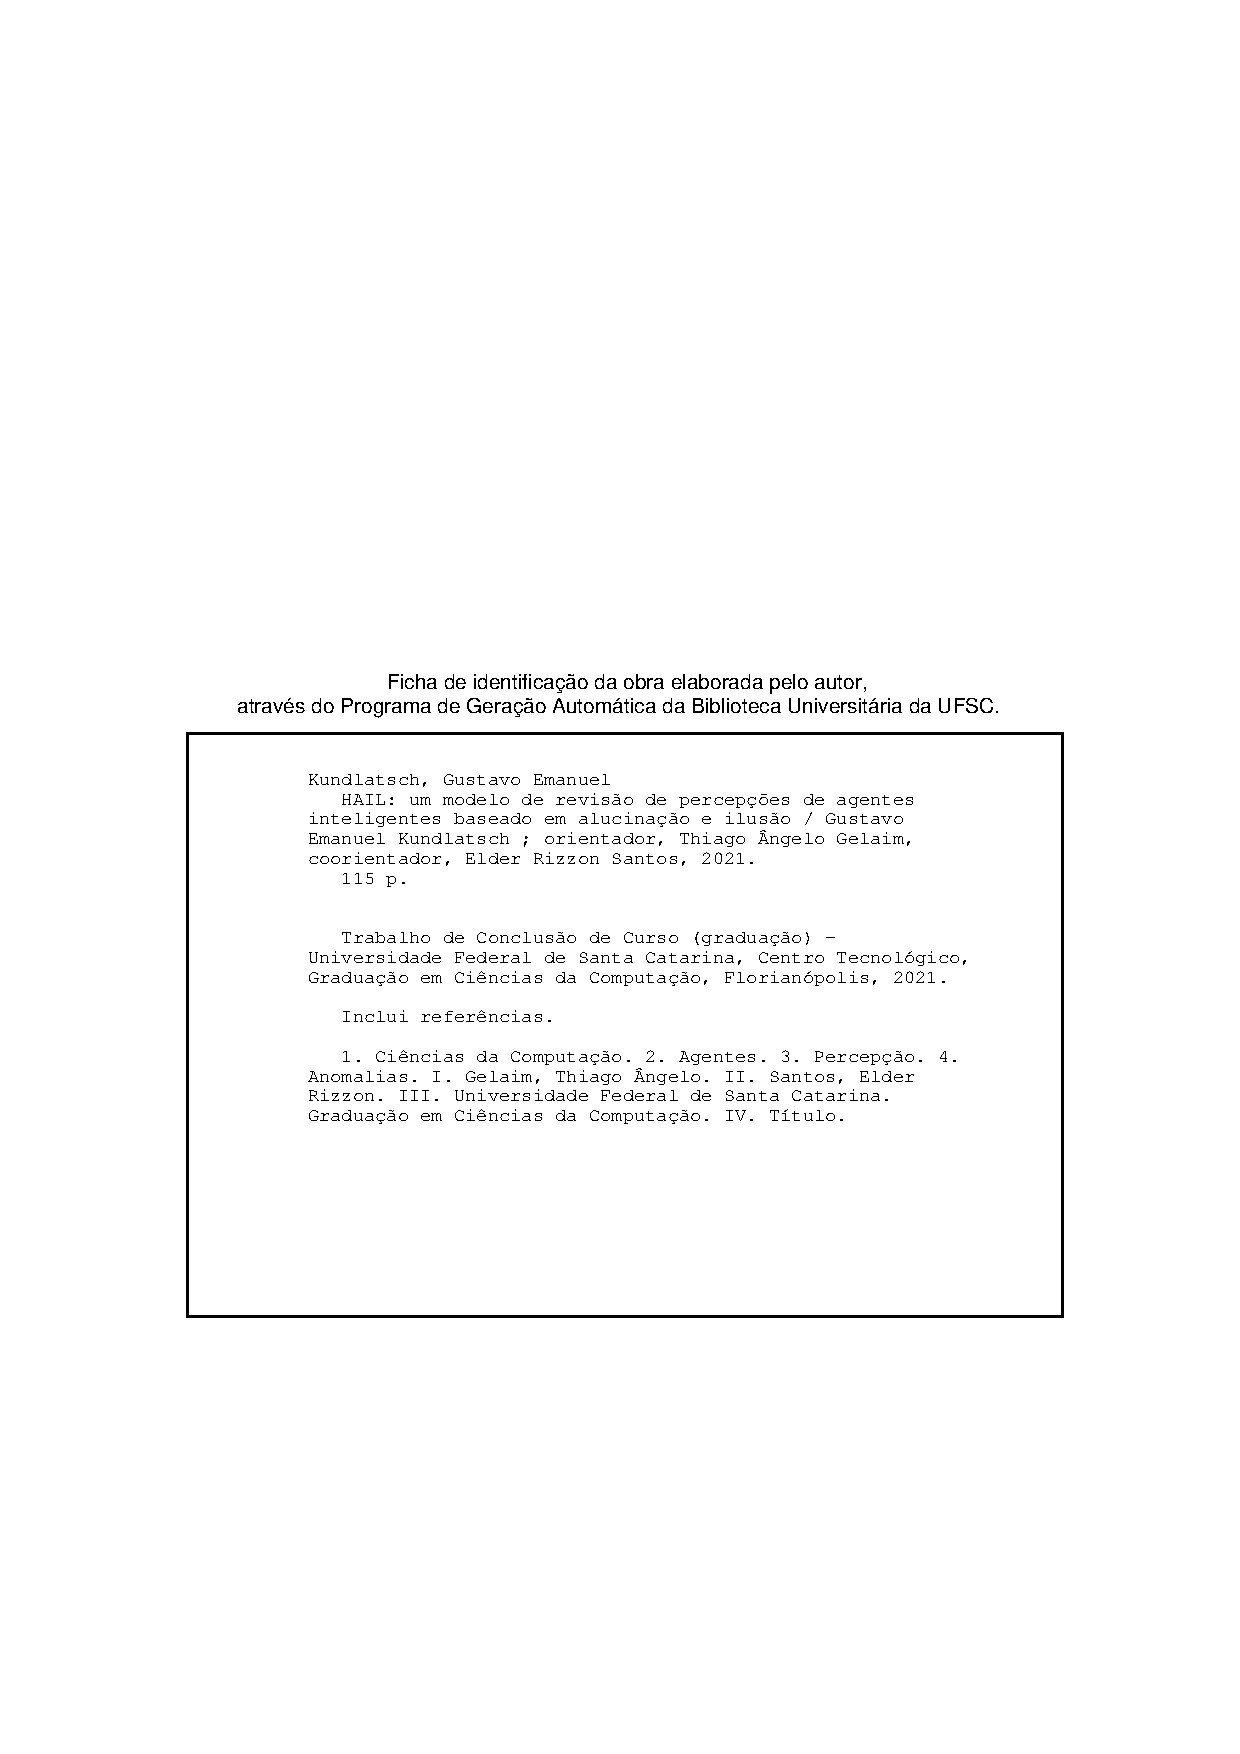
\includepdf{beforetext/Ficha_Catalografica.pdf}
\end{fichacatalografica}
% ---

% ---
% Inserir folha de aprovação
% ---
\begin{folhadeaprovacao}
	\OnehalfSpacing
	\centering
	\imprimirautor\\%
	\vspace*{10pt}		
	\textbf{\imprimirtitulo}%
	\ifnotempty{\imprimirsubtitulo}{:~\imprimirsubtitulo}\\%
	%		\vspace*{31.5pt}%3\baselineskip
	\vspace*{\baselineskip}
	%\begin{minipage}{\textwidth}
	O presente trabalho em nível de \imprimirnivel~foi avaliado e aprovado por banca examinadora composta pelos seguintes membros:\\
	%\end{minipage}%
	\vspace*{\baselineskip}
	Dr. Thiago Ângelo Gelaim\\
	Orientador\\
	\vspace*{\baselineskip}
	Prof. Dr. Elder Rizzon Santos \\
	Coorientador e Responsável\\
	\vspace*{\baselineskip}
	Prof. Dr. Rafael de Santiago\\
	\vspace*{\baselineskip}
	Me. Rodrigo Rodrigues Pires de Mello\\
	\vspace*{2\baselineskip}
	\begin{minipage}{\textwidth}
		Certificamos que esta é a \textbf{versão original e final} do trabalho de conclusão que foi julgado adequado para obtenção do título de \imprimirformacao.\\
	\end{minipage}
	%    \vspace{-0.7cm}
	\vspace*{\fill}
	\assinatura{\OnehalfSpacing Coordenação do Programa de Graduação}
	\vspace*{\fill}
	\assinatura{\OnehalfSpacing\imprimirorientador \\ \imprimirorientadorRotulo}
	%	\ifnotempty{\imprimircoorientador}{
	%	\assinatura{\imprimircoorientador \\ \imprimircoorientadorRotulo \\
	%		\imprimirinstituicao~--~\imprimirinstituicaosigla}
	%	}
	% \newpage
	\vspace*{\fill}
	\imprimirlocal, \imprimirano.
\end{folhadeaprovacao}
% ---

% ---
% Dedicatória
% ---
\begin{dedicatoria}
	\vspace*{\fill}
	\noindent
	\begin{adjustwidth*}{}{5.5cm} 
		\raggedleft       
		Para meus pais, que sempre souberam que o melhor investimento para os filhos é a educação.
	\end{adjustwidth*}
\end{dedicatoria}
% ---

% ---
% Agradecimentos
% ---
\begin{agradecimentos}

    Quando fazemos uma escolha, ela recebe o peso de toda a potencialidade morta das alternativas que não foram escolhidas. Sou muito grato a minha família, que sempre me deu toda a liberdade do mundo para tomar minhas próprias escolhas e que também sempre me apoiou, no acerto ou no erro, independente da dificuldade enfrentada. Eu escolhi cursar computação, e mesmo que minha família não entenda muito bem o que isso significa, sempre esteve comigo me incentivando a seguir meus sonhos.

	Este trabalho não representa o ciclo final de minha graduação, mas todo o caminho trilhado nesses anos de curso. Ele é resultado de um processo que começou no fim do meu primeiro semestre, um processo que me fez conhecer muitas pessoas incríveis e que me desenvolveu tanto profissionalmente quanto como pessoa. O laboratório sempre foi para mim uma forma de expressar minha criatividade, e esta monografia é resultado de apenas uma das muitas ideias que eu tive. Por essa liberdade de criar e por todas as reuniões de orientação que tive ao longo desses anos eu agradeço ao professor Elder e ao Thiago, que tiveram a paciência de me acolher na minha iniciação científica.
	
	A maior benção que recebi na vida foram meus amigos, e não posso deixar de agradecê-los aqui. Seja para jogar, reclamar da vida, chorar as mágoas ou simplesmente desfrutar da companhia uns dos outros, meus amigos nunca me deixaram na mão. Eu sempre quis ser um contador de histórias, e compartilhar meus causos com meus amigos, distribuindo sorrisos e gargalhadas, é algo que dinheiro nenhum no mundo seria capaz da comprar.
	
	Por fim, gostaria de agradecer cada servidor da UFSC e profissional da comunidade, que são responsáveis pela alimentação, limpeza e organização de nossa universidade pública e gratuita. Sem o trabalho de cada uma dessas pessoas, essa conquista não seria possível.

\end{agradecimentos}
% ---

% ---
% Epígrafe
% ---
\begin{epigrafe}
	\vspace*{\fill}
	\begin{flushright}
		\textit{``Qualquer lugar é o paraíso desde que queira viver.\\
		    Afinal, todos estão vivos.\\
		    E, enquanto for assim, todos têm chance de ser feliz.''\\
			(Anno, End of Evangelion, 1997)}
	\end{flushright}
\end{epigrafe}
% ---

% ---
% RESUMOS
% ---

% resumo em português
\setlength{\absparsep}{18pt} % ajusta o espaçamento dos parágrafos do resumo
\begin{resumo}
	\SingleSpacing
	Percepções são a principal maneira de uma entidade receber informações do ambiente. Cada pessoa possui uma maneira diferente de perceber e interpretar o mundo. Entretanto, sabe-se que na percepção humana existem anomalias, que são percepções incorretas que enganam a mente. Dito isso, como podemos saber se nossas percepções são reais ou se são apenas fruto de nossa imaginação? E a questão derivada disso é: e computadores? Agentes inteligentes são entidades computacionais autônomas capazes de tomar decisões baseadas no ambiente no qual estão inseridos, e utilizam sensores para reconhecerem o mundo a sua volta. Mas esses sensores podem falhar. Neste trabalho, apresentamos um modelo genérico de revisão de percepções, capaz de tratar anomalias recebidas pelo agente e criar novos planos a partir delas para se adaptar ao ambiente. Esse modelo foi implementado e submetido a experimentos para testar seu funcionamento. As simulações realizadas demonstraram que o modelo é capaz de detectar e classificar as anomalias, e que em ambientes com grande quantidade de percepções inválidas o modelo consegue ter maior impacto criando novos planos através do planejamento automatizado e aumentando a quantidade de percepções válidas recebidas pelo raciocínio do agente.
	
	\textbf{Palavras-chave}: Agentes. Percepção. Anomalias.
\end{resumo}

% resumo em inglês
\begin{resumo}[Abstract]
	\SingleSpacing
	\begin{otherlanguage*}{english}
		Perceptions are the primary way for an entity to receive information from the environment. Each person has a different manner of percept and interpret the world. However, it is known that in human perception, there are anomalies, incorrect perceptions that deceive the mind. So, how can we know if our perceptions are real or just tricks from our minds? Furthermore, the follow-up question is: what about computers? Intelligent agents are computational entities capable of making decisions based on the environment and use sensors to perceive the world. However, sensors can fail. In the current work, we present a generic model of perception revision, capable of treating anomalies received by the agent and creating new plans to adapt to the environment. This model was implemented and submitted to experiments to test its behaviour. The simulations demonstrate that the model is capable of detecting and classifying anomalies. In environments with a high amount of invalid perceptions, the model can have more impact creating new plans through the automatic planning process and increasing the number of valid perceptions received by the agent's cognition.
		
		\textbf{Keywords}: Agents. Perception. Anomalies.
	\end{otherlanguage*}
\end{resumo}
%% resumo em francês 
%\begin{resumo}[Résumé]
% \begin{otherlanguage*}{french}
%    Il s'agit d'un résumé en français.
% 
%   \textbf{Mots-clés}: latex. abntex. publication de textes.
% \end{otherlanguage*}
%\end{resumo}
%
%% resumo em espanhol
%\begin{resumo}[Resumen]
% \begin{otherlanguage*}{spanish}
%   Este es el resumen en español.
%  
%   \textbf{Palabras clave}: latex. abntex. publicación de textos.
% \end{otherlanguage*}
%\end{resumo}
%% ---

{%hidelinks
	\hypersetup{hidelinks}
	% ---
	% inserir lista de ilustrações
	% ---
	\pdfbookmark[0]{\listfigurename}{lof}
	\listoffigures*
	\cleardoublepage
	% ---
	
	% ---
	% inserir lista de quadros
	% ---
	\pdfbookmark[0]{\listofquadrosname}{loq}
	\listofquadros*
	\cleardoublepage
	% ---
	
	% ---
	% inserir lista de tabelas
	% ---
	\pdfbookmark[0]{\listtablename}{lot}
	\listoftables*
	\cleardoublepage
	% ---
	
	
	% ---
	% inserir lista de abreviaturas e siglas (devem ser declarados no preambulo)
	% ---
	% ---------------------------------------------------
% ------ Lista de abreviaturas e siglas -------------
% ---------------------------------------------------

\begin{siglas}
  \item[ BDI ] \hspace{0.7cm} \emph{Belief-Desire-Intention}
  \item[ EOM ] \hspace{0.7cm} \textit{Environment Object Model}
  \item[ IA ] \hspace{0.7cm} Inteligência Artificial
  \item[ K-CoPMan ] \hspace{0.4cm} \textit{Knowledge enabled Cognitive Perception for Manipulation}
  \item[ NPC ] \hspace{0.7cm} Número de Percepções recebidas por Ciclo
  \item[ OA-SMTRNN ] \textit{Object Augmented Supervised Multiple Timescale Recurrent}
  
  \hspace{0.7cm} \textit{Neural Network}
  \item[ PDDL ] \hspace{0.7cm} \textit{Planning Domain Definition Language}
  \item[ PMK ] \hspace{0.7cm} \textit{Perception and Manipulation Knowledge}
  \item[ PPI ] \hspace{0.7cm} Porcentagem de Percepções Inválidas
  \item[ RP ] \hspace{0.7cm} Relação Percentual
  \item[ SMA ] \hspace{0.7cm} Sistema Multiagente
  \item[ TMA ] \hspace{0.7cm} Tempo Médio gasto pelo planejamento Automatizado
  \item[ TMC ] \hspace{0.7cm} Tempo Médio gasto em um Ciclo de raciocínio
\end{siglas}
	% ---
	
	% ---
	% inserir lista de símbolos (devem ser declarados no preambulo)
	% ---
	% ---------------------------------------------------
% ----------- Lista de símbolos ---------------------
% ---------------------------------------------------

\begin{simbolos}
  \item[$ \Delta $] Função de transição do modelo de revisão de percepções
  \item[$ \Gamma $] Função de transição que especifica um sistema de transição de estados $\Sigma$
  \item[$ \gamma $] Função de percepção do agente
  \item[$ \theta $] Função de refinamento
  \item[$ \rho $] Conjunto de percepções refinadas
  \item[$ \Sigma $] Sistema de transição de estados de um modelo conceitual de planejamento automatizado
  \item[$ \Psi $] Conjunto união formado pelas pré-condições das ações que compõem um plano
  \item[$ \psi $] Conjunto de pré-condições de uma ação
  \item[$ \Omega $] Conjunto união formado pelas pós-condições das ações que compõem um plano
  \item[$ \omega $] Conjunto de pós-condições de uma ação
  \item[$ A $] Conjunto finito ou recursivamente enumerável de ações
  \item[$ Ab $] Conjunto de blocos avaliadores
  \item[$ Ab_{h} $] Bloco avaliador de alucinações
  \item[$ Ab_{i1} $] Bloco avaliador de ilusões classe 1
  \item[$ Ab_{i2} $] Bloco avaliador de ilusões classe 2
  \item[$ Ag$ ] Agente
  \item[$ Ap $] Conjunto de blocos de planejamento automatizado
  \item[$ Ap_{h} $] Bloco de planejamento automatizado de alucinações
  \item[$ Ap_{i} $] Bloco de planejamento automatizado de ilusões
  \item[$ c $] Contexto do agente
  \item[$ Ce $] Função equação de limpeza do bloco avaliador
  \item[$ Cf $] Função de limpeza do bloco avaliador
  \item[$ D $] Conjunto de decisores
  \item[$ d_{a} $] Decisor de anomalias
  \item[$ d_{h} $] Decisor de alucinações
  \item[$ d_{i} $] Decisor de ilusões
  \item[$ E $] Conjunto finito ou recursivamente enumerável de eventos
  \item[$ K $] Conjunto de conhecimentos do agente
  \item[$ L $] Lista ordenada
  \item[$ |L| $] Número de elementos de uma lista ordenada
  \item[$ L_i $] Elemento $i$ da lista ordenada $L$
  \item[$ M_{ai} $] Módulo de alucinação e ilusão
  \item[$ P $] Conjunto de planos do agente
  \item[$ p $] Conjunto de percepções iniciais
  \item[$ P(L_i) $] Função peso da lista ponderada
  \item[$ Pf $] Função de processamento do bloco avaliador
  \item[$ S $] Conjunto finito ou recursivamente enumerável de estados
  \item[$ T_{m}(x) $] Função tempo médio de x
  \item[$ W $] Função peso de uma anomalia
  \item[$ Z $] Descrição de sistema
\end{simbolos}


	% ---
	
	% ---
	% inserir o sumario
	% ---
	\pdfbookmark[0]{\contentsname}{toc}
	\tableofcontents*
	\cleardoublepage
	
}%hidelinks
% ---
% ---

% ----------------------------------------------------------
% ELEMENTOS TEXTUAIS
% ----------------------------------------------------------
\textual

\chapter{Introdução}

Dentro da Inteligência Artificial (IA), agentes inteligentes são entidades capazes de raciocinar a respeito do ambiente em que estão inseridos e tomar decisões baseadas na situação em que se encontram \cite{russell2016artificial}. Dessa maneira, podemos descrever um agente pelos seus processos de percepção, raciocínio e atuação. O agente ocupa um ambiente, do qual recebe informações e no qual atua. O ambiente é o mundo em que o agente está inserido, podendo ser virtual ou uma parte do mundo real, no caso de um agente físico. Existem diversos tipos de ambientes que podem ser classificados de acordo com o seu fechamento (que determina se agentes de fora do ambiente podem afetar o sistema), dinamismo (a maneira como o ambiente evolui), determinismo (a consistência dos efeitos no ambiente) e cardinalidade (o número de objetos a serem afetados e percebidos) \cite{moya2007towards}.

Uma das maneiras de um agente atualizar seu conhecimento a respeito do ambiente é a percepção, o processo de utilizar sensores para detectar o ambiente e transformar os dados coletados em informações úteis \cite{weyns2004towards}.  O raciocínio, por sua vez, é o processamento das percepções baseado nos objetivos do agente, que resulta em um conjunto ações a serem tomadas através dos atuadores. O processo do raciocínio é comandado pela arquitetura cognitiva do agente, um modelo computacional inspirado na estrutura da mente humana \cite{DYACHENKO2018130}. As arquiteturas cognitivas podem ser divididas em três categorias: simbólicas, emergentes e híbridas \cite{yeCognitivearchitectures}. Arquiteturas simbólicas descrevem o ambiente através de símbolos armazenados em memória em uma base de conhecimentos, e utilizam lógica simbólica para realizar o ciclo de percepção, raciocínio e ação. Arquiteturas emergentes se baseiam na estrutura biológica do cérebro e normalmente utilizam redes neurais em uma estrutura hierárquica para lidar com situações de incerteza. Por fim, arquiteturas híbridas combinam o comportamento emergente e o processamento simbólico para resolver problemas de diversos domínios. 

Todavia, sensores podem apresentar problemas para o processo de percepção por razões como campo de visão, distância do objeto observado, resolução dos sensores e leituras não confiáveis \cite{chrisman1991intelligent}. Tratar deste problema normalmente é responsabilidade da arquitetura cognitiva do agente, pois a arquitetura precisa ser capaz de fazer a ponte entre o ambiente e o conhecimento do agente \cite{langley2009cognitive}.

O objetivo deste trabalho é apresentar um modelo genérico (independente da arquitetura do agente) que pode ser acoplado entre o processo de percepção e raciocínio, capaz de detectar e tratar percepções inválidas para transformá-las em informações úteis através de um processo de criação de novos planos. Esse modelo pressupõe um ambiente aberto (onde agentes externos podem influenciar o ambiente), dinâmico (mudanças no ambiente são causadas por eventos aleatórios) e não determinístico (ações do agente causam resultados diferentes no ambiente, mesmo em situações aparentemente idênticas, pois os resultados variam dependendo da percepção do agente daquele evento).  Com isso, buscamos responder as perguntas de pesquisa:

\begin{itemize}
    \item Como podemos diferenciar percepções válidas de percepções inválidas?
    \item Como podemos utilizar percepções inválidas para criar novos planos?
\end{itemize}

\iffalse

Agentes são baseados em arquiteturas cognitivas, \emph{frameworks} criados para simular a cognição humana \cite{newell1994unified}.

Um exemplo de arquitetura cognitiva é o modelo \emph{belief-desire-intention} (BDI), originado na psicologia com a teoria do raciocínio prático de Bratman \cite{bratman1987intention}, posteriormente implementado como um modelo computacional por Rao \cite{rao1995bdi}. No BDI, os estados internos do agente são divididos em crenças, desejos e intenções. Crenças são todo o conhecimento que o agente possui a respeito do mundo, recebidos da percepção do ambiente e de comunicações com outros agentes ou outras fontes externas. Desejos são as mudanças que o agente deseja causar no mundo, e as intenções representam os estados deliberativos do agente, ou seja, coisas que o agente efetivamente se dispôs a fazer.



\fi


\section{Justificativa}

Para que um agente possa interagir com o ambiente, ele precisa atualizar seus estados internos, de acordo com regras estabelecidas por sua arquitetura cognitiva. A percepção é a capacidade do agente sentir o mundo, resultando em uma expressão que por si própria pode ser entendida e interpretada \cite{wyens2004}. Em ambientes dinâmicos, há possivelmente centenas de percepções por segundo \cite{hayes1992guardian}. Mas percepções não necessariamente precisam incluir representações corretas da realidade e podem variar de agente para agente \cite{janssen2005agent}. Um agente com percepção incompleta pode ter problemas de percepções por conta de limitações de sua capacidade de perceber determinados objetos ou obstrução física dos sensores, por exemplo \cite{chrisman1991intelligent}. 

Falhas na entrada de dados através de sensores pode ser perigoso, levando o agente a tomar decisões incorretas, especialmente caso o agente faça parte de um sistema crítico. Por exemplo, em um sistema controlado por um agente cujo objetivo é trocar a cor do semáforo sempre que detectar pedestres o suficiente vindo de diversas direções, o mal funcionamento de um sensor pode levar a cor do semáforo a trocar com muita frequência, trancando os carros e levando a um grande engarrafamento -- ou pior, pode causar o atropelamento de um pedestre.

Para categorizar as percepções incorretas e diferenciá-las das percepções válidas, foram utilizados dois conceitos vindos do estudo de percepção da filosofia: (i) alucinações, que são percepção completamente válidas, mas que ocorrem em um momento errado e (ii) ilusões, percepções ou de objetos existentes no ambiente com características incorretas, ou de objetos inexistentes no ambiente mas com características comuns a objetos válidos \cite{perception-problem}.

Com base no nome em inglês desses dois conceitos foi definido o nome do modelo proposto neste trabalho: HAIL (\textit{hallucination} e \textit{illusion}, alucinação e ilusão em inglês, respectivamente).

\section{Objetivos}

\subsection{Objetivo geral}

Este trabalho possui como objetivo geral propor um modelo de revisão de percepções capaz de detectar percepções inválidas e transformá-las em informações úteis para o agente.

\subsection{Objetivos específicos}

\begin{enumerate}
    \item Analisar o estado da arte relativo a percepções de agentes inteligentes;
    \item Criar um modelo capaz de detectar, classificar e aprender com percepções inválidas;
    \item Formalizar e implementar o modelo proposto em um ambiente genérico (sem contexto de aplicação);
        \item Testar o modelo proposto através de diferentes simulações, utilizando o design fatorial de experimentos. 
\end{enumerate}

\section{Organização do trabalho}

Este trabalho está organizado do seguinte modo:

\begin{itemize}
    \item O capítulo 2 apresenta e define formalmente a fundamentação teórica necessária para a compreensão do trabalho, dentre eles inteligência artificial, agente inteligente, percepção e planejamento automatizado;
    \item O capítulo 3 é um compilado de alguns trabalhos relacionados, que exploram o problema de percepções inválidas de diferentes maneiras;
    \item O capítulo 4 apresenta e define formalmente o modelo HAIL;
    \item O capítulo 5 descreve os experimentos realizados para testar o modelo HAIL e apresenta seus resultados;
    \item O capítulo 6 contém as considerações finais e os trabalhos futuros.
\end{itemize}

\chapter{Conceitos Fundamentais}

%\input{Content/trabalhos.tex}
Neste capítulo, serão apresentado os conceitos fundamentais utilizados para o desenvolvimento do trabalho. Ele apresenta os conceitos básicos de inteligência artificial e um estudo aprofundado sobre agentes e percepções. Além disso, nesse capítulo são definidos os conceitos básicos que serão utilizados na construção do modelo apresentado nos capítulos seguintes.

\section{Inteligência Artificial}

A inteligência artificial (IA) é um campo de estudo intrigante pois diferente de outros campos do conhecimento que se limitam a buscar entender \textit{como} o pensamento humano funciona, a IA se propõem a construir entidades pensantes \cite{russel2013artificial}. Apesar da IA ser uma área de pesquisa que surgiu a quase setenta anos, não existe uma única definição de inteligência artificial nem consenso dentro da comunidade acadêmica.

Bellman define inteligência artificial como a automatização de diversas tarefas humanas: ``atividades que associamos ao pensamento humano, atividades como a tomada de decisões, a resolução de problemas, o aprendizado''. Ele chega nessa definição a partir da pergunta ``computadores podem pensar?''. o autor desmembra tal indagação em diversos exemplos de atividades que os computadores são capazes de executar, como os descritos anteriormente além de outros conceitos, como incerteza, conciência e humor. A conclusão de Bellman, apesar disso, é que ``O espírito humano se mantém muito acima de qualquer coisa que possa ser automatizada'' \cite{bellman1978introduction}. Essa é uma visão de que o objetivo da inteligência artificial é replicar o pensamento humano.

Outro ponto de vista é o de Charniak e McDermott, que definem inteligência artificial como ``O estudo das faculdades mentais através do uso de modelos computacionais'' \cite{charniak1985introduction}. Essa definição é interessante pois para ela ser correta é necessário que exista uma equivalência entre o processo mental humano e o processamento de um computador. Por conta disso, tais autores definem o dogma central da inteligência artificial: ``O que o cérebro faz pode ser pensado em algum nível como um tipo de computação''. Para eles, caso o dogma se mostre verdadeiro, o uso de modelos computacionais para o estudo das faculdades mentais é valido. ``Faculdades mentas'', dentro dessa definição, são os mecanismos internos que recebem imagens e palavras (através da visão e da linguagem) e os converte em saídas na forma de ações robóticas e fala. Esse processamento interno inclui dedução, planejamento, aprendizado e outras técnicas.

Russel separa as definições de inteligência artificial entre aquelas que defendem que os computadores devem pensar como humanos, e aquelas que defendem que os computadores devem agir como humanos \cite{russel2013artificial}. As duas definições apresentadas anteriormente estão no primeiro grupo. Entretanto, as definições que levam em conta que os computadores devem agir como humanos em geral possuem um aspecto mais prático. Por exemplo, a definição de Rich e Knight diz que inteligência artificial é ``o estudo de como os computadores podem desempenhar tarefas que hoje são melhor desempenhadas pelas pessoas'' \cite{rich1991artificial}. Com isso podemos notar que esse lado mais prático da IA não se precisa se preocupar tanto com as questões filosóficas por trás do pensamento humano, pois foca em resolver problemas reais através dos métodos existentes. 

Para o trabalho atual, utilizaremos uma definição nessa mesma linha de pensamento de que o computador deve agir como um ser humano, nesse caso específico, de maneira lógica. Para Poole, ``inteligência computacional é o estudo do desenvolvimento de agentes inteligentes'' \cite{poole1998computational}. Essa definição nos é interessante pois esse trabalho se trata de um modelo desenvolvido para agentes inteligentes. A sessão seguinte desse capítulo se dedica a definir o que é um agente.

Independente da definição utilizada, podemos afirmar que a inteligência artificial é um campo vasto que intriga muitos pesquisadores. Esse campo possui diversas técnicas, que são utilizadas para resolver todo o tipo de problemas. Kurzweil possui uma visão bastante interessante sobre a pesquisa de inteligência artificial:

\begin{displayquote}
    É nosso destino como pesquisadores de inteligência artificial nunca alcançar a cenoura pendurada à nossa frente. A inteligência artificial é inerentemente definida como a busca de problemas difíceis da ciência dos computadores que ainda não foram resolvidos. \cite{kurzweil2000age}
\end{displayquote}



\section{Agente}

Um agente inteligente é uma entidade autônoma, capaz de tomar as próprias decisões. Apesar da definição intuitiva ser simples, assim como no termo inteligência artificial, não existe um consenso da comunidade sobre o que é um agente. Russel e Norving definem agente simplesmente como algo que age, e agente inteligente como aquele que age buscando o melhor resultado possível \cite{russel2013artificial}. Poole segue a linha de que é uma entidade que atua no ambiente em que está inserido. O autor descreve:

\begin{displayquote}
    Um agente inteligente é um sistema que age de maneira inteligente: o que faz é apropriado para as circunstâncias e seus objetivos, é flexível para mudar ambientes e mudar objetivos, aprende com a experiência e faz escolhas apropriadas, dadas as limitações perceptivas e a computação finita \cite{poole1998computational}.
\end{displayquote}

Tais definições são bastante amplas, e enquadram diversos tipos de programas computacionais. Apesar disso, agentes possuem características específicas, principalmente provenientes da capacidade de interagir uns com os outros. Luger apresenta cinco tópicos que demonstram as capacidades e características dos agentes inteligentes \cite{lugerBook6th}:

\begin{enumerate}
    \item \textbf{Agentes são autônomos ou semi-autônomos:} Os agentes são independentes, ou seja, cada agente é capaz de trabalhar em uma tarefa sem saber no que outros agentes estão trabalhando, ou sem saber como eles resolvem determinada tarefa. Além disso, eles podem tanto fazer algo efetivamente (agir) ou reportar seus resultados para outros agentes (se comunicar).
    \item \textbf{Agentes possuem escopo localizado:} Cada agente é sensível ao ambiente, e normalmente não possui conhecimento sobre aquilo que todos os outros agentes estão realizando. Portanto o conhecimento de um agente é limitado às tarefas que ele deve realizar, sem conhecimento amplo sobre seus limites.
    \item \textbf{Agentes são interacionais:} Normalmente, agentes se agrupam em forma de sociedade, com o objetivo de colaborar para resolver um problema. E assim como na sociedade humana, o conhecimento, a responsabilidade, habilidades e outros recursos estão distribuídos entre os indivíduos.
    \item \textbf{As sociedades dos agentes são estruturadas:} Na maioria das abordagens de solução de problema orientada a agentes, cada agente, mesmo possuindo seu próprio conjunto de habilidades e objetivos, se coordena com outros agentes para a resolução geral de problemas. Portanto, a solução final não é apenas coletiva, mas também cooperativa.
    \item \textbf{O fenômeno da inteligência nesses ambientes é emergente:} A capacidade final da resolução de um problema por uma sociedade de agentes é maior do que a soma das capacidades individuais de trabalho. A inteligência é vista como um fenômeno residente e emergente de uma sociedade e não apenas uma propriedade de um agente individual.
    
\end{enumerate}

Woolbridge e Jennings distinguem a noção de agente como podendo ser forte ou fraca \cite{wooldridge1995intelligent}. A noção fraca de agente é utilizada para denominar hardware ou software que possui algumas características específicas, sendo elas autonomia, habilidade social, reatividade e pró-atividade. Já a noção forte de agente se refere a um sistema que, além das características citadas anteriormente, ou foi concebida ou foi implementada utilizando conceitos que normalmente se aplicam a humanos. O modelo explorado nos capítulos seguintes segue a noção forte de agente, pois se baseia em conceitos da psicologia e da filosofia para resolver um problema prático dos agentes.

Com base na leitura das definições apresentadas anteriormente, para este trabalho vamos definir agente formalmente conforme apresentado abaixo, de maneira que facilite a manipulação e formalização do modelo proposto.

\theoremstyle{definition}
\begin{definition}
    \label{def:agent}
    Um agente é uma tripla $Ag = \langle K, P, \gamma \rangle$, onde:
    \begin{itemize}
        \item $K$ é conjunto de conhecimentos que o agente possui, tal que $K = \emptyset \cup K_i \cup K_p \cup K_c$, onde $K_i$ é o conjunto de conhecimentos inicias do agente, $K_p$ os conhecimentos adquiridos através das percepções e $K_c$ os conhecimentos adquiridos através de comunicações;
        \item $P$ é o conjunto de planos do agente, sendo um plano definido como $plan = (pre, A, pos)$, onde $pre$ é o conjunto união formado com as pré condições das ações que compõem o plano, $A$ o conjunto de ações que compõe o plano e $pos$ o conjunto união formado com as pós condições das ações que compõem o plano. Por sua vez, uma ação é definida como $action = (pre, n, pos)$, sendo $pre$ um conjunto de pré condições, $n$ um nome para a ação e $pos$ um conjunto de pós condições; e
        \item $\gamma$ é a função de percepção, definida como $ \gamma: p \times K \rightarrow P $, onde $p$ é o conjunto de percepções recebidas pelo agente.
    \end{itemize}{}
\end{definition}{}

A partir dessa definição, podemos construir o conceito de contexto, que será amplamente utilizado na formalização do modelo de revisão de percepções. O contexto de um agente é o conjunto de todos os símbolos compreendidos pelo agente, e cuja percepção de cada um desses símbolos resulta na execução de um conjunto de ações diretamente mapeadas.

\begin{definition}
    O contexto $c$ de um agente $Ag$ é o domínio de sua função $\gamma$.
    \label{definition::context}
\end{definition}{}



\iffalse
\section{Agente}

Essa seção é um esqueleto de uma definição de agente que pode ser útil para explicar o modelo proposto. O foco é a relação da função $\Lambda$ com o resto do modelo, portanto K, A e P precisam ser melhorados.

Para esse artigo vamos definir agente como a quádrupla $Ag = (K, A, P, \Lambda)$, onde:

\begin{itemize}
    \item K é o conjunto de conhecimentos que o agente possui, podendo ter adquirido ou já ter começado com eles. Essas conhecimentos podem se referir a coisas que o agente conhece do mundo, coisas que o agente quer mudar no mundo ou coisas abstratas.
    \item A é o conjunto de atuadores do agente, ou seja, coisas que o agente pode usar para causar mudança no mundo (e, portanto, nos conhecimentos K).
    \item P é o conjunto de percebedores do agente, que adquirem novas informações a respeito do ambiente, causando mudança em K.
    \item $\Lambda$ é a função de percepção, que opera sobre a entrada de P, baseado nas informações contidas em K e retorna um subconjunto de A.
    \[ \Lambda: P \times K \rightarrow 2^A\]
\end{itemize}

Eu não sei se o jeito que eu escrevi está certo, mas usando essa ideia o que foi chamado de Contexto no resto do artigo pode ser facilmente definido como a imagem da função $\Lambda$.

\fi

\section{Percepção}

Existem diversas definições para o termo ``percepção''. Gibson propõem que, fundamentalmente, podemos entender percepção como um conjunto de sensações que, através da maneira subjetiva que um dado agent o interpreta, representa determinadas entidades do ambiente \cite{gibson1950perception}. Ou seja, a percepção não é simplesmente a representação direta das entidades reais que existem no mundo, mas um processo complexo que varia para cada indivíduo.

Chalmers et. al. divide a percepção nos níveis baixo e alto \cite{chalmers1992high}. A percepção de baixo nível ocorre através de meios físicos, os órgãos ópticos para os humanos ou os sensores para os agentes. A percepção de alto nível aparece no momento e que \textit{conceitos} começam a ter um papel importante, e pode ser divida em diversas faculdades, como o reconhecimento de objetos e o relacionamento entre entidades. Nos trabalhos de inteligência artificial, em geral, estamos interessados na percepção de alto nível, pois a percepção de baixo nível está mais relacionada a robótica (agentes que possuem hardware próprio) ou a simulação (agentes que possuem apenas software).

Ainda segundo Chalmers et. al. uma das principais características da percepção de alto nível é a extrema flexibilidade. Um mesmo objeto do ambiente pode ser percebido de diversas maneiras, de acordo com as características do observador. Para os autores, alguma das fontes da flexibilidade das percepções são a capacidade de serem influenciadas pelas crenças, objetivos e contexto externo. Além disso, percepções de um mesmo objeto podem ser radicalmente alteradas conforme o necessário.

Para o modelo que iremos propor, baseado na definição \ref{def:agent}, o conceito de percepção pode ser simplesmente definido como as entradas da função de percepção $\gamma$ de um agente. Vale destacar a diferença entre percepção e contexto, pois o contexto é constituído pelas percepções que fazem parte do domínio da função $\gamma$.

Em ambientes dinâmicos, há possivelmente centenas de percepções por segundo \cite{hayes1992guardian}. Mas percepções não necessariamente precisam incluir representações corretas da realidade e podem variar de agente para agente \cite{janssen2005agent}. Um agente com percepção incompleta pode ter problemas de percepções por conta de limitações de sua capacidade de perceber determinados objetos ou obstrução física dos sensores, por exemplo \cite{chrisman1991intelligent}.

\subsection{Refinamento}

Como o volume de percepções de um agente pode ser muito grande, e as percepções tomam determinado tempo para serem processadas, é interessante reduzirmos o volume de percepções que chegam ao ciclo de raciocínio do agente. Em nosso modelo, esse processo será chamado de refinamento, e ocorre entre o momento que as percepções são recebidas pelos sensores e a entrada de dados no modelo proposto por nós. Portanto, iremos definir refinamento da seguinte maneira:

\begin{definition}
    \label{def:refinamento}
    Refinamento de percepções é uma função $\theta$ tal que, dado o conjunto de entradas de percepções $p$, reduz tais percepções para um subconjunto próprio $\rho$.
\end{definition}

Existem deiversas maneiras de realizar refinamento. Uma das mais clássicas é o uso de filtros de percepções, que limitam que percepções serão processados pelo agente baseado em diversos critérios, como posição, distância e a velocidade do objeto percebido \cite{bordeux2001}. Outra maneira de restringir as percepções é a percepção ativa. Aloimonos et. al. \cite{Aloimonos1988} define um observador como ativo se ele ativamente pode  executar uma ação que altere as configurações geométricas de seus sensores, com objetivo de melhorar a qualidade de sua observação. Bajcsy et. al. \cite{Bajcsy2018} descreve um \emph{framework} completo para implementar a percepção ativa através da tupla por quê, o que, quando, onde e como perceber. Desta maneira, o agente pode perceber apenas quando é necessário (por quê), escolhendo o que perceber (o que) e otimizar fisicamente a percepção (quando, onde e como).

\subsection{Anomalias}

Anomalias são o foco principal deste trabalho. Usaremos a seguinte definição:

\begin{definition}
    Uma percepção $p$ de um agente $Ag$, é uma anomalia caso $p \notin c$ de $Ag$.
\end{definition}

Ou seja, toda percepção para a qual o agente não tenha uma resposta mapeada em sua função de percepção, é uma anomalia. O conjunto de anomalias pode ser definido também como o conjunto de percepções possíveis que não fazem parte do contexto de um dado agente.

Anomalias podem ser divididas em dois tipos: alucinações e ilusões. Nas seções seguintes, será descrito o que ilusões e alucinações são para os estudos clássicos do problema da percepção \cite{Russell1912-RUSTPO-49} \cite{Price1933-PRIP-20}, e também apresentaremos nossa definição computacional que será utilizada mais tarde. A base desse estudo foi o artigo ``The Problem of Perception'', de Crane et. al. \cite{perception-problem}

\subsection{Ilusão}

Uma ilusão, na definição clássica onde o objeto de estudo são os seres humanos, é qualquer situação perceptiva na qual um objeto físico é realmente percebido, mas ele aparenta ser outra coisa que ele não é \cite{Smith2002-SMITPO-17}. Para deixar mais claro o que é uma ilusão, vamos utilizar um exemplo.

%Essa definição será usada como base para criar nossa definição computacional para ilusão. Entretanto, é importante notar que essa é uma definição diferente de outras encontradas na literatura, como a usada por Lhelani et. al. \cite{Khemlani2017}, onde uma ilusão é uma falácia advinda de uma interpretação humana errada sobre um problema lógico resolvido pelo computador.

\begin{example}{}
Suponha um robô que possui a tarefa de empacotar diferentes itens do depósito de uma loja. Os itens passam por uma esteira, e o agente usa dois sensores para perceber o que os itens são. O primeiro sensor é uma câmera ligada ao topo do corpo do robô, usado para definir a forma do item. O segundo sensor é um detector de textura na lateral das esteiras. Assim, as informações advindas dos sensores formam predicados da forma \texttt{forma(textura)}, que descreve um item. Os itens podem ter as forma de um círculo, um quadrado ou um triângulos, e a textura lisa ou listrada.
O agente possui duas cores de papéis para empacotar, vermelho e azul. O papel vermelho é usado para quadrados (de ambas as texturas) e círculos lisos. O papel azul é usado para círculos listrados e triângulos lisos. A loja não vende triângulos listrados, então não há nenhum item desse tipo no depósito. Podemos descrever esse comportamento com as seguintes regras:

\begin{center}
    \texttt{papel(vermelho) :- quadrado(\_) OR circulo(liso)}
\end{center}
\begin{center}
     \texttt{papel(azul) :- circulo(listrado) OR triangulo(liso)}
\end{center}

\begin{figure}[h!]
    \centering
    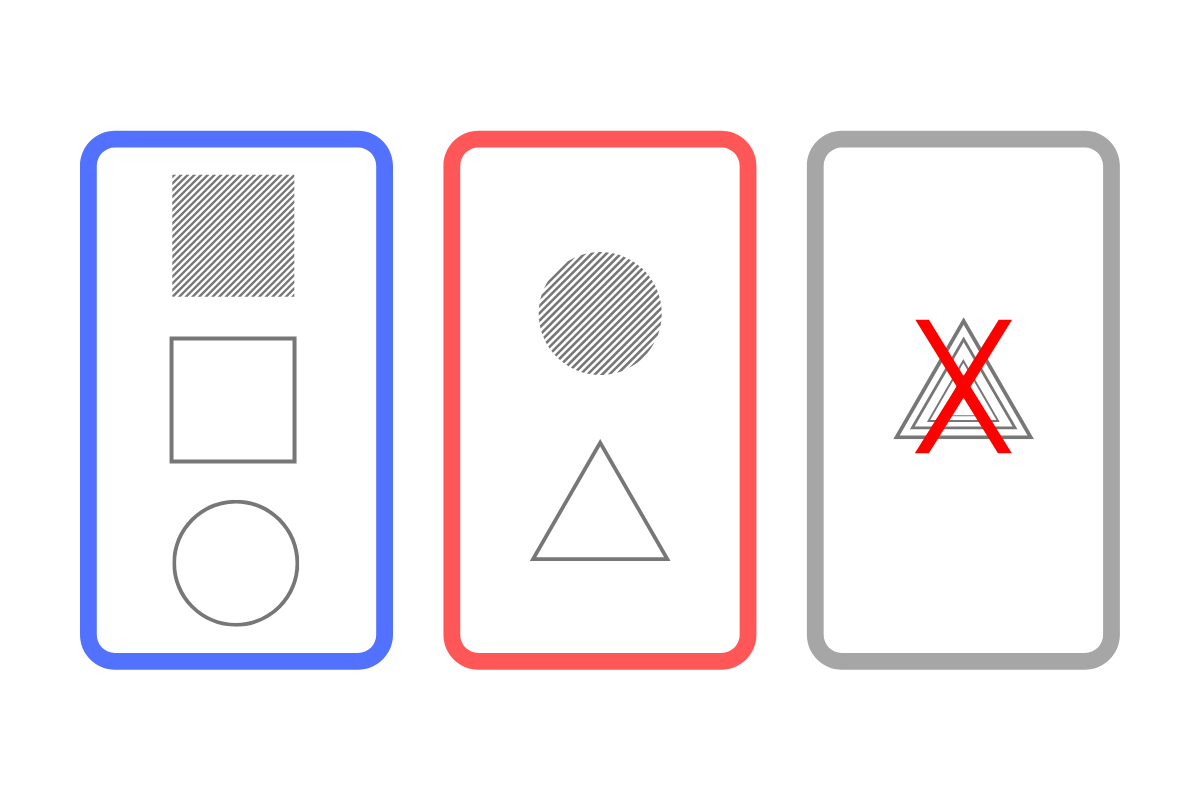
\includegraphics[width=0.45\textwidth]{Images/img1}
    \caption{Funcionamento do agente empacotador.}
    \label{fig:method}
\end{figure}
\label{example::robo}
\end{example}

\begin{example}
Agora vamos estender o exemplo \ref{example::robo} supondo que o sensor tátil não está funcionando corretamente, e ele irá sentir objetos lisos como se fossem ondulados. Para nosso exemplo, vamos considerar que o primeiro item será um triângulo liso. Nenhum erro ocorre quando a câmera percebe o triângulo, mas o sensor tátil indica que ele é ondulado. Nesse caso, teremos uma ilusão, pois triângulo é um objeto válido, mas ele foi percebido com uma propriedade inválida, que não existe no contexto do agente. Não há planos para quando o agente detecta esse tipo de erro, então ele pode executar um plano padrão para casos de erro, ou simplesmente não fazer nada.
\label{example::ilusao1}
\end{example}{}

Esse tipo de anomalia demonstrado no exemplo \ref{example::ilusao1} será chamado de ilusão classe 1, onde o corpo do predicado, ou o objeto da percepção, é válido, mas possui um argumento ou uma característica inválida.

\begin{definition}{}
   Uma ilusão classe 1 é uma percepção do tipo \texttt{objeto(caracteristica)} ou equivalente, onde \texttt{objeto} é um elemento do contexto do agente e \texttt{característica} não é.
\end{definition}

\begin{example}
    Se considerarmos que as percepções do agente possuem formas erradas por conta de um defeito na câmera ou o software de reconhecimento de padrões que atua sobre ela, um objeto como um círculo liso pode ser reconhecido como um estrela listrada. Estrela não é um objeto válido, mas listrado é.
    \label{example::ilusao2}
\end{example}{}

Isso será chamado de ilusão classe 2, definido de maneira similar a ilusão classe 1.

\begin{definition}{}
   Uma ilusão classe 2 é uma percepção do tipo \texttt{objeto(caracteristica)} ou equivalente, onde \texttt{objeto} não é um elemento do contexto do agente e \texttt{característica} é.
\end{definition}

Portanto, podemos simplesmente definir ilusão da seguinte forma:

\begin{definition}{}
   Uma ilusão é uma percepção do tipo \texttt{objeto(caracteristica)} ou equivalente, que se caracteriza como uma ilusão classe 1 ou uma ilusão classe 2.
\end{definition}

\subsection{Alucinação}

\begin{example} {}
    Retornando ao exemplo \ref{example::ilusao1} do agente responsável por empacotar os itens, mas que agora apresenta também o comportamento defeituoso do exemplo \ref{example::ilusao2}. Uma percepção formalmente correta, do tipo \texttt{objeto(caracteristica)}, por conta dos erros que os sensores possurm podem resultar na percepção \texttt{estrela(ondulada)}. Essa percepção poderia ser processada pelo agente, entretanto ela não faz parte de seu contexto, e cairia também em algum plano padrão para casos de erro ou simplesmente não executar nada.
    \label{exemple::alucinacao}
\end{example}

Assim, uma alucinação é um tipo específico de ilusão classe 1 e classe 2, podendo acarretar os mais diversos tipos de erros dentro do raciocínio do agente, ou gerando problemas caso seja ignorada. Portanto, uma alucinação pode ser definida da seguinte maneira:

\begin{definition}{}
   Uma alucinação é uma percepção do tipo \texttt{objeto(caracteristica)} ou equivalente, onde nem \texttt{objeto} nem \texttt{característica} é um elemento do contexto do agente.
\end{definition}

\section{Planejamento Automatizado}

Planejamento automatizado é um dos problemas fundamentais da inteligência artificial. As motivações para usar o planejamento automatizado são a capacidade de utilizar recursos de planejamento acessíveis e eficientes e reproduzir uma parte do processo cognitivo humano com um componente totalmente integrado de comportamento deliberativo\cite{GHALLAB20041}. A maneira clássica de realizar planejamento automatizado era considerar esse um problema de dedução lógica, onde era dado um estado inicial, ações que aferam esse estado e um conjunto de estados de objetivo, e era necessário encontrar a sequência de ações que faziam com que o ambiente saísse de um estado inicial para um estado de objetivo \cite{MADANI20035}.

Uma forma alternativa de tratar o problema de planejamento automatizado é utilizando planejamento probabilístico. Essa abordagem pode ser necessária por conta do fato de que o agente provavelmente não tem conhecimento completo do mundo ao seu redor. Kushmerick et. al. apresenta um modelo utilizando esse conceito \cite{KUSHMERICK1995239}. Outra saída para o problema do planejamento automatizado, utilizada por outros autores (e. g. \cite{Cassandra:1998:EAA:926710}, \cite{DBLP:journals/corr/abs-1105-5460}, \cite{article}), são os processos de decisão de Markov. O modelo que iremos apresentar não exige uma implementação específica de planejamento automático, ficando a cargo da implementação tomar a decisão de que caminho seguir. 

Abaixo, apresentamos a definição abstrata de planejamento automático, descrita como um modelo conceitual simples que contém os elementos principais do problema, tendo sido originalmente apresentada por Ghallab et. al. \cite{GHALLAB20041}.

\begin{definition}{}
\label{definition::autoplanning}
   % USAR MAIS TARDE PARA DEFINIR O BLOCO DE AUTOPLANEJAMENTO An automated planning block is a instance of the conceptual model of automated planning, described through the interaction between three components bellow \cite{GHALLAB20041}:
   Um modelo conceitual de planejamento automatizado é descrito como a interação entre os seguintes três componentes:
   
    \begin{itemize}
        \item Um sistema de transição de estados $\Sigma$, especificado por uma função de transição de estados $y$, de acordo com os eventos e ações que ele recebe. 
        \item Um $controlador$, que dado uma entrada de estados $s$ do sistema, fornece como saída uma ação de acordo com algum plano.
        \item Um $planejador$, que dado uma entrada de uma descrição de sistema $Z$, uma situação inicial e alguns objetivos, sintetiza um plano para o controlador a fim de alcançar o objetivo.
    \end{itemize}
    
    Um sistema de transição de estados $\Sigma$ é uma quádrupla $\Sigma = \langle S, A, E, \Gamma \rangle$, onde:
    
    \begin{itemize}
        \item $S = \{s_1, s_2, ..., s_{n}\}$ é um conjunto finito ou recursivamente enumerável de estados;
        \item $A = \{a_1, a_2, ..., a_{n}\}$ é um conjunto finito ou recursivamente enumerável de ações;
        \item $E = \{e_1, e_2, ..., e_{n}\}$ é um conjunto finito ou recursivamente enumerável de eventos; e 
        \item $\Gamma: S \times A \times E \rightarrow 2^S$ é uma função de transição de estados. 
    \end{itemize}
     
\end{definition}
% \chapter{Trabalhos Relacionados}
\chapter{Trabalhos relacionados}

\label{chapter:relacionados}

Existem diversas abordagens para otimizar as percepções recebidas por um agente, isto é, garantir que todas as informações coletadas pelos sensores sejam utilizadas da melhor maneira possível. Diversos artigos sobre o assunto, com diferentes abordagens, são publicados todos os anos. Para definir os trabalhos relacionados apresentados nessa seção, foram utilizados diversos termos de busca, uma vez que os termos ilusão e alucinação podem não necessariamente se aplicarem às percepções da mesma maneira definida neste trabalho.

Nos mecanismos de busca Google Scholar e Scopus foram realizadas pesquisas que associam agentes inteligentes a percepções inválidas, anomalias ou ilusões e alucinações, além de termos auxiliares como aprendizado e otimização. As buscas aconteceram ao longo do desenvolvimento do trabalho, e diversas \textit{strings} de busca foram utilizadas e combinadas. Conforme encontraram-se os artigos, suas introduções foram verificadas para averiguar se o conteúdo realmente estava relacionado ao processo de revisão de percepções. Depois disso foi realizada uma leitura inicial dos trabalhos selecionados, e os quatro mais adequados foram escolhidos para um estudo mais profundo.

Os artigos apresentados nas Seções \ref{van2011} e \ref{diab2019} implementam modelos para tratar de percepções em ambientes onde é possível receber percepções que não são totalmente confiáveis, semelhante ao conceito de anomalia definido no Capítulo \ref{conceitos-fundamentais}. Os artigos das Seções \ref{pangercic2010} e \ref{kim2017} são trabalhos relacionados a outros campos de estudo de percepção, mas que precisam resolver problemas relacionados a percepções imperfeitas. A maneira como esses artigos se conectam ao modelo proposto no trabalho atual está descrita em mais detalhes nas seções seguintes.

\section{Scalable perception for BDI-agents embodied in virtual environments \cite{van2011scalable}}

\label{van2011}
Ambientes virtuais como jogos, simulações e treinamentos exigem cada vez mais complexidade dos agentes com os quais os participantes interagem. A arquitetura BDI (\textit{belief-desire-intension}) provê a complexidade necessária para que os agentes virtuais desempenhem as tarefas avançadas necessárias. Porém, agentes BDI tradicionais possuem uma interface direta com o ambiente, enquanto os agentes dos jogos normalmente possuem um conjunto de sensores limitados para realizar suas percepções. O problema é que agentes BDI não possuem um mecanismo padrão para controlar seus sensores, decidindo quais percepções receber. Dessa maneira, o agente pode facilmente ficar sobrecarregado de informação. Para resolver esse problema, os autores desse trabalho criaram um \textit{framework} que fornece habilidades sensoriais e e atenção perceptiva para agentes BDI incorporados em um ambiente virtual, funcionando como um \textit{middleware} que atua entre o modelo cognitivo do agente e o ambiente.

Nesse \textit{framework} (representado na figura \ref{fig:bdiPerceptionModel}) toda informação do ambiente é representada pelo modelo de informação chamado \textit{Environment Object Model} (Modelo de Objeto de Ambiente) ou EOM. Objetos são definidos por classes e características, e existe uma hierarquia de objetos para agregar semântica. O \textit{middleware} é dividido entre a interface física e a interface cognitiva. A função da interface física é interagir com o ambiente para formar símbolos. Para tal, o processador sensorial primeiro recebe uma lista de possíveis percepções, que respeita filtros predeterminados implementados nos sensores. Após isso, esse processador determina se o agente está interessado nas informações recebidas, através do \textit{Interest Subscription Manager} (gerenciador de inscrição de interesse). Estes símbolos são passados para o agente na foma de percepções, que alteram os objetivos do agente. Os novos objetivos, por sua vez, são repassados para o sistema de atenção, que atualiza os interesses do agente no gerenciador de inscrição de interesse. A comunicação entre a interface física e a interface cognitiva é realizada através de mensagens, e há interfaces para que o \textit{middleware} possa se comunicar com o ambiente e com o agente, de maneira a mantê-lo independente de domínio. 

\begin{figure}[h!]
    \centering
    \caption{\textit{Framework} de percepção baseado em EOM.}
    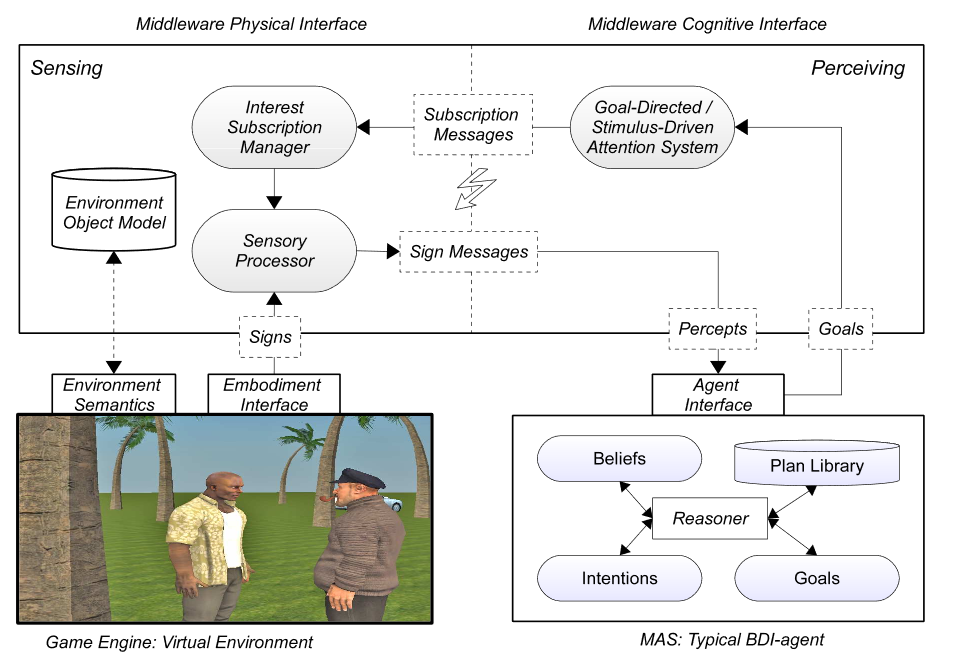
\includegraphics[width=\textwidth]{images/bdiPerceptionModel.png}
    \legend{Fonte: Scalable perception for BDI-agents embodied in virtual environments \cite{van2011scalable}.}
    \label{fig:bdiPerceptionModel}
\end{figure}

Para avaliar o modelo proposto, foram realizados dois experimentos. O primeiro consistiu no uso de sensores físicos em um teste de estresse, tanto em um sistema que utilizava o framework quando em um que não o utilizava. As percepções recebidas pelos agentes continham cinco atributos cada, sendo que a quantidade de entidades percebidas aumentava gradativamente. Cinco baterias de testes foram conduzidas para cada agente. O segundo experimento consistiu na implementação de um sistema multiagente (SMA) de agentes BDI baseado em Java e utilizando uma engine Prolog para realizar o raciocínio, e os mesmos testes do primeiro experimento foram realizados.

Esse modelo, que é capaz de decidir que tipo de percepções o agente deseja perceber de acordo com seus interesses, se assemelha ao HAIL porque muda dinamicamente ao longo do tempo, conforme as percepções são processadas. Além disso, ele possui um elemento de percepção ativa, pois o conjunto de percepções recebidas de maneira direta e massiva do ambiente é filtrado pelo processador de sensores.


\section{PMK — a knowledge processing framework for autonomous robotics perception and manipulation \cite{Diab_2019}}

\label{diab2019}
As tarefas executadas por robôs vêm se tornando cada vez mais complexas. Para realizar essas tarefas, os robôs precisam passar por uma etapa de planejamento, na qual decidem quais ações tomar baseados no estado atual do ambiente ao seu redor. Alguns dos mecanismos clássicos de planejamento utilizam a Linguagem de Definição de Domínio de Planejamento (\textit{Planning Domain Definition Language} ou PDDL) para descrever o ambiente no qual o agente está inserido. O problema é que essa abordagem assume um mundo fechado, i.e., que todos os fatos sobre o mundo são conhecidos, caso contrário o planejador pode falhar. Com essa limitação, um robô não é capaz de começar uma tarefa a não ser que todos os objetos do ambiente tenham sido reconhecidos e as ações que ele deve executar tenham sido definidas. Em outras palavras, a existência de alucinações e ilusões limita o funcionamento de tais sistemas.

Para resolver esse problema em situações onde o robô precisa realizar tarefas complexas de manipulação, foram criadas abordagens de planejamento baseadas no conhecimento, que utilizam reconhecimento semântico do cenário, conhecimento a respeito do comportamento físico de objetos e raciocínio sobre as possíveis ações de manipulação.

O trabalho de Diab et al. propõem um \textit{framework} de representação de conhecimento baseado em ontologias (uma especificação formal de conhecimento) chamado PMK (\textit{Perception and Manipulation Knowledge}), apresentado na figura \ref{fig:pmk}. Esse modelo é genérico, para que possa ser utilizado em diversos domínios, e incorporado com outras ontologias. O PMK permite associar dados de percepção de baixo nível (proveniente dos sensores, na camada física do sistema) com conhecimento de alto nível (camada de raciocínio do agente).
Uma dos principais contribuições do artigo é criar um \textit{framework} que funcione como uma caixa preta para um planejador qualquer: o PMK é capaz raciocinar sobre os recursos do robô, suas restrições de ação, a viabilidade de ação e os comportamentos de manipulação. Para isso, o modelo utiliza análise situacional, avaliando a situação a situação dos objetos no ambiente com base em posicionamento espacial, acessibilidade do robô aos objetos, potencial área na qual o objeto será colocando entre outros. 

A abordagem que é proposta pelo PMK oposta ao HAIL, pois tenta mapear todas as percepções possíveis em baixo nível a priori. Dessa forma, mesmo que o agente não tenha sido projetado para tratar determinadas percepções, ele é capaz de entender o significado semântico delas através do \textit{framework}. Em outras palavras, a ideia do PMK é criar um mapa extenso para que nenhuma percepção recebida pelo agente seja uma anomalia.

\begin{figure}
    \centering
    \caption{\textit{Framework} PMK.}
    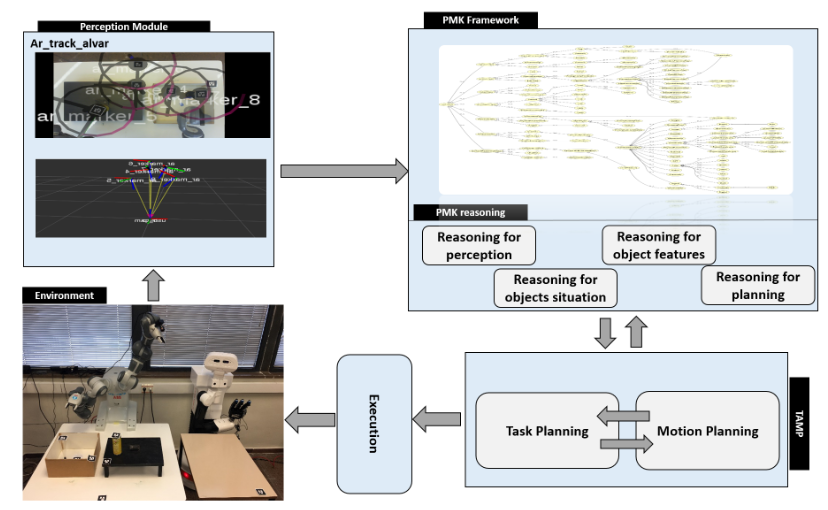
\includegraphics[width=0.9\textwidth]{images/pmk-model.png}
    \legend{Fonte: PMK - a knowledge processing framework for autonomous robotics perception and manipulation \cite{Diab_2019}.}
    \label{fig:pmk}
\end{figure}

\section{Combining perception and knowledge processing for everyday manipulation \cite{pangercic2010}}

\label{pangercic2010}
Robôs autônomos implementados para realizar tarefas de manipulação de objetos do dia a dia precisam tomar diversas decisões que requerem a combinação de percepção e processamento de conhecimento. Esse artigo de Panger et al. apresenta um sistema de programação lógica chamado K-CoPMan (\textit{Knowledge enabled Cognitive Perception for Manipulation}, ou Percepção Cognitiva Ativada pelo Conhecimento para Manipulação). Esse modelo é capaz de testar e satisfazer pré-condições de conhecimento para manipulações do dia a dia. Para isso, ele fornece ao agente o conhecimento simbólico abstrato sobre as cenas percebidas, usa conhecimento simbólico abstrato para realizar tarefas de percepção e responde a novos tipos de consultas que exigem a combinação de percepção e processamento de conhecimento.

Um dos principais mecanismos do K-CoPMan é o componente de percepção passiva. Para se tornar consciente do ambiente, o agente que utiliza tal sistema pode escanear a cena em busca de áreas de interesse, como mesas ou cadeiras, utilizar os sensores para detectar objetos. Cada objeto recebe um identificador único, para então ser guardado na base de conhecimentos, juntamente com o contexto do momento em que a percepção foi realizada. O identificador é utilizado para que mais tarde seja possível examinar mais a fundo objeto, e possivelmente classificá-lo ou categorizá-lo. Portanto, o K-CoPMan permite que agentes inteligentes estejam conscientes do ambiente ao seu redor fazendo uma varredura completa do ambiente, uma vez que utiliza tanto percepção ativa quanto passiva, e guardando as anomalias detectadas para que possam ser tratadas mais tarde por um módulo próprio (o servidor de percepção).

A abordagem desse trabalho para evitar os efeitos de percepções inválidas é similar ao PMK, mas ao invés de utilizar uma base de conhecimentos prévia para evitar que alguma percepção não possa ser tratada pelo agente, o próprio sistema cria sua base através da varredura do ambiente pela percepção passiva.

\section{Understanding human intention by connecting perception and action learning in artificial agents \cite{kim2017understanding}}

\label{kim2017}
Para desenvolver agentes capazes de realizar comportamentos complexos similares aos de seres humanos, é primeiro preciso entender como os seres humanos aprendem a perceber, pensar e agir em um mundo dinâmico. Diversos campos da inteligência artificial buscam replicar esses comportamentos, além de outros como a emoção e a cooperação. Essas habilidades parecem ser intrínsecas aos seres humanos, e tornam nossas relações mútuas únicas. Em particular, a capacidade de entender a intenção dos outros tem sido considerada a base da comunicação entre humanos. Nesse artigo, Kim, Yu e Lee propõem um modelo, chamado OA-SMTRNN (\textit{Object Augmented Supervised Multiple Timescale
Recurrent Neural Network}), para entender a intenção do usuário e responder ativamente da maneira mais adequada, através do uso de redes neurais. Para implementar o reconhecimento de intenção, são focados dois processos cognitivos, a percepção da disponibilidade de objetos e a previsão da ação humana.

Nos experimentos realizados pelos autores, diversos objetos precisaram ser percebidos pelo agente. Entretanto, alguns objetos poderiam estar sobrepostos, conforme demonstra a Figura \ref{fig:overlap}. Nesses casos, as percepções recebidas pelo agente poderiam estar incorretas. Para resolver este problema, o módulo responsável pelas ações foi implementado com a capacidade de relacionar a ação e os objetos. No artigo, é exemplificada a relação entre ``encher um copo d'água'' e ``fazer um café mocha''. Ou seja, o modelo, que foi previamente treinado, se mostrou capaz de associar a intenções como ``beber leite'' a determinadas ações (segurar um objeto, leva algo para a boca) para inferir que determinada anomalia (uma caixa de leite sobreposta por uma caneca) era uma caixa de leite.

\begin{figure}[h!]
    \centering
    \caption{Exemplo de sobreposição de imagens na percepção.}
    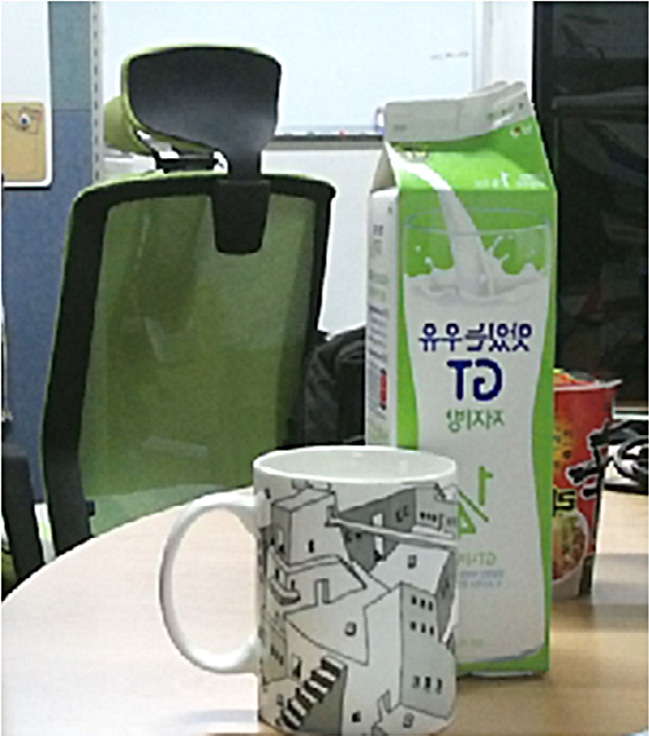
\includegraphics[width=0.5\textwidth]{images/overlap.jpg}
    \legend{Fonte: Understanding human intention by connecting perception and action learning in artificial agents \cite{kim2017understanding}.}
    \label{fig:overlap}
\end{figure}

Enquanto no modelo de revisão de percepções apresentado buscamos resolver o problema de percepção de anomalias através de uma abordagem simbólica, que classifica, trata e aprende com ilusões e alucinações, o modelo OA-SMTRNN utiliza uma abordagem conexionista, com o uso de redes neurais, para conseguir extrair semântica de percepções que seriam inicialmente inválidas para o agente. Além disso, na conclusão do trabalho é mencionado que “implementar aprendizagem de percepção-ação conectada pode desempenhar um papel importante no desenvolvimento de agentes artificiais que podem inferir a intenção humana e interagir melhor”. No HAIL, essa integração é realizada uma vez que as anomalias percebidas são utilizadas pelos módulos de planejamento automatizado para criar novos planos.

\section{Discussão}

Os quatro trabalhos que foram selecionados possuem diversas similaridades e diferenças. Para visualizar isso melhor, eles foram separados de acordo com as seguintes categorias, para então comporem o Quadro \ref{tab:relacionados}:

\begin{enumerate}
    \item Apresenta ou não um \textit{framework} genérico que pode ser aplicado em qualquer agente, independente de arquitetura;
    \item A abordagem que o trabalho utiliza para tratar percepções inválidas: limitando as percepções, de maneira que o agente realize a percepção apenas sobre as entidades que ele está pronto para tratar; definindo o ambiente, através de alguma forma de representação de conhecimento que descreve o mundo do agente para que ele possa tratar todas as percepções recebidas; ou tratar as anomalias recebidas através de algum sistema que processa as percepções inválidas recebidas;
    \item Tipos de experimentos realizados: se foram feitas simulações de software ou se foi construído um agente físico para testar o modelo;
    \item Tipos de percepções que o agente recebia: completas, no caso de ambientes simulados, ou físicas, no caso de agentes físicos;
    \item Forma de avaliação que foi utilizada para mensurar a eficácia do método proposto;
    \item Paradigma do agente (simbólico ou conexionista);
    \item Se o modelo apresenta ou não alguma ferramenta de aprendizado que utiliza ilusões e alucinações para gerar novos planos ou conhecimento.
\end{enumerate}

Através dessa classificação, é possível destacar em quais pontos nosso modelo se assemelha e diverge dos trabalhos relacionados que foram selecionados. O principal referencial do HAIL está no processo de revisão de percepções simbólico e na capacidade de permitir que qualquer arquitetura possua um processo de aprendizagem através do planejamento automatizado. Isso se reflete principalmente na forma de avaliação (tempo de processamento, como no trabalho \ref{van2011}, e também pela taxa de aprendizado do modelo) e no tipo de percepção utilizada nos experimentos (completas, pois o agente recebe a informação diretamente da simulação, mas sem semântica atrelada e sem contexto de aplicação). Além disso, três dos quatro trabalhos selecionados possuem um ambiente físico no mundo real: os trabalhos \ref{diab2019} e \ref{pangercic2010} na forma de implementação física e o trabalho \ref{kim2017} na forma de percepção de imagens que foram extraídas de um ambiente real. Isso é um indicativo de que trabalhos futuros podem implementar nosso modelo fisicamente, em robôs, por exemplo.

\begin{landscape}

% \usepackage{colortbl}


\begin{quadro}[]
\caption{Trabalhos relacionados categorizados.}
 \makegapedcells
\begin{tabular}{|P{2.3cm} |P{2.5cm}|P{2.5cm}|P{3cm}|P{2.5cm}|P{3.5cm}|P{2.3cm}|P{2.5cm}|}
\hline

\textbf{Trabalho}       & \textbf{Framework Genérico} & \textbf{Abordagem} & \textbf{Experimentos}                 & \textbf{Tipos de Percepções}                       & \textbf{Forma de Avaliação}                        & \textbf{Paradigma} & \textbf{Ferramenta de Aprendizado} \\ \hline
OIJEN; DIGNUM, 2011     & Sim (BDI)                   & Limitar percepções & Simulação de SMA com ambiente gráfico & Completas (semântica no ambiente)                  & Tempo de processamento                             & Simbólico          & Não                                \\ \hline

DIAB et al., 2019       & Sim                         & Definir o ambiente & Implementação física                  & Física (câmeras)                                   & Corretude da tarefa executada                      & Simbólico          & Não                                \\ \hline
Pangercic et. al., 2010 & Não                         & Definir o ambiente & Implementação física                  & Física (câmeras)                                   & Corretude da tarefa executada                      & Simbólico          & Não                                \\ \hline

KIM; YU; LEE, 2017      & Não                         & Tratar anomalias   & Implementação de modelo computacional & Dataset de imagens                                 & Corretude da predição                              & Conexionista       & Sim                                \\ \hline
\textbf{HAIL (trabalho atual)}          & \textbf{Sim}                         & \textbf{Tratar anomalias}   & \textbf{Simulação de agente único}             & \textbf{Completas (aleatórias e independentes de contexto)} & \textbf{Tempo de processamento e capacidade de aprendizado} & \textbf{Simbólico}          & \textbf{Sim}                                \\ \hline
\end{tabular}
 \label{tab:relacionados}
 \legend{Fonte: Autor.}
\end{quadro}

\end{landscape}


\iffalse
\newpage
\section{SEÇÃO DE TRABALHOS RELACIONADOS (ORGANIZAÇÃO)}

Essa seção estão conteúdos ligados a pesquisa de trabalhos relacionados, mas será movida ou distribuída no artigo final.

\begin{itemize}
    \item O trabalho de John Anderson [9] propõem uma versão distribuída do simulador de agentes únicos Gensim. No artigo, Anderson discorre sobre como colocar a fonte das percepções completamente dentro do agente ou do ambiente é filosoficamente impreciso. Além disso, o autor descreve como isso também representa um problema prático, uma vez que a preparação sensorial é um elemento computacionalmente intensivo, portanto um equilíbrio deve ser encontrado.
    
    \item Para Włodzisław Duch [10], em seu trabalho sobre inteligência computacional, um dos grandes problemas atuais dessa área é seu foco em raciocínio como computação, e o uso da lógica como base do raciocínio, deixando de lado o caráter técnico de como símbolos precisam primeiro serem derivados de percepções reais. Segundo o autor, o cérebro humano é altamente especializado em análise de padrões naturais e outras técnicas que permitem o mapeamento de percepções a ações, mas apesar do grande avanço na área de inteligência computacional, sistemas projetados para resolver essas funções cognitivas de ordem inferior ainda estão muito distantes da capacidade do cérebro biológico.
    
    \item Bordeux et. al. [8] apresenta uma pipeline de percepção para agentes autônomos, propondo um processo de pré-processamento, processamento e pós-processamento utilizando filtros de percepções. filtro de agente, composto por um filtro de percepção, opcionalmente um filtro semi-reflexivo (que não será discutido por estar fora do escopo do trabalho atual) e uma lista de objetos selecionados. A ideia de guardar a lista de objetos selecionados conversa com o bloco avaliador de nosso modelo, pois guarda informações de determinadas percepções realizadas para serem mais tarde reaproveitadas para um ajuste fino.
    
    \item Em um artigo de revisão sobre arquiteturas cognitivas, Langley et. al [3] caracteriza a importância de tratar de percepções imperfeitas, e mostra que as arquiteturas podem conter elementos para tratar disso, uma vez que os sensores geralmente possuem interferências ou outros tipos de ruídos, que afetam a qualidade da percepção obtida. Segundo o autor, ambientes dinâmicos complicam ainda mais a situação, uma vez que o agente precisa rastrear alterações que ocorrem muitas vezes de maneira repentina no ambiente. A única solução que o autor propõem a isso é o “conhecimento perceptivo”, onde o agente decide sobre quais sensores utilizar, onde e quando focaliza-los e que interferências são plausíveis, se aproximando da percepção ativa.
    
    \item Mesmo em simulações virtuais, às percepções podem levar a erros por conta de sua imprecisão. Sichman [6] ilustra alguns aspectos essenciais de mecanismos de raciocínio sociais, baseado na noção de dependência social. O sistema proposto trata de um modelo de coalizões, onde agentes podem se juntar em prol de um objetivo em comum. O protocolo de formação de coalizões é formado por proposições, aceitações, recusas e mensagens de revisão. As mensagens de revisão são necessárias pois uma possível razão para um agente se recusar a participar de uma coalizão é porque o remetente tem uma crença falsa sobre suas capacidades, ou seja, acreditar que o agente pode executar uma ação, mas na realidade não pode. Isso pode acontecer pois fontes de informação, como as percepções, podem levar a erros.

    \item O trabalho de Pangercic et. al. [7] trata de percepção e processamento de conhecimento, usando como estudo de caso um robô encarregado de determinar quais objetos faltam em uma mesa durante uma refeição, através de inferências lógicas. A implementação resulta em um modelo estatístico, em que cada objeto que o robô conhece recebe uma porcentagem de chance de ser necessário. Apesar dessa alta volatilidade, os autores não tratam da possibilidade da inferência incorreta.
    
    \item Diab et. al. apresenta um framework de processamento de conhecimento para a manipulação de percepção de robôs autônomos, através de raciocínio de percepção, isto é, raciocínio relacionado às características perceptivas dos objetos no ambiente, como outros modelos também fazem, mas além disso adiciona raciocínio relacionado aos algoritmos que o sensor pode executar para extrair os recursos, aos sensores associados ao robô e as limitações físicas dos sensores. Segundo os autores, esse processo torna o robô mais inteligente e flexível. Essa flexibilidade pode ser útil para lidar com a falhas de um sensores, fornecendo alternativas, ou seja, o framework proposto tem flexibilidade para lidar com sistemas sensoriais de vários modelos.
    
\end{itemize}

\textbf{Problema abordado no artigo:} Conforme abordado pelo artigo [3], interferências ocorrem entre o processo físico de percepção e o processamento final dela, dentro do ciclo cognitivo do agente. Portanto, esse trabalho ataca essa lacuna que existe, com o objetivo de minimizar percepções incorretas ou falhas completas de percepção.

\textbf{Contribuição do artigo:} Nesse artigo é apresentado um modelo genérico para o tratamento de percepções, com o objetivo de evitar que informação potencialmente útil seja desperdiçada, criando novos planos quando o agente não está pronto para lidar com percepções que estão fora do seu planejamento inicial. Esse modelo foi construído para que possa ser acoplado a qualquer arquitetura cognitiva, independente do grau de abstração que ela implemente.

\textbf{fim da seção de organização dos trabalhos relacionados}
\fi
\chapter{Modelo de Revisão de Percepções}

\noindent O modelo proposto para revisão de percepção é separado em três etapas, como mostra a figura \ref{fig:method}. Primeiro, o agente recebe um conjunto de percepções $p$ através de seus sensores. Depois disso, essas percepções passam através de uma função de refinamento, onde as percepções $p$ são refinadas tornando-se um subconjunto próprio $\rho$ de percepções refinadas. O conjunto $\rho$ é então passado para o módulo de alucinação e ilusão, onde cada percepção refinada passa por um processo de detecção de anomalia. As percepções de $\rho$ que forem consideradas válidas, irão constituir o subconjunto próprio $\varrho$ de percepções válidas, enquanto as anomalias formarão o subconjunto próprio $\sigma$ de anomalias. As percepções válidas são enviadas direto para o ciclo de raciocínio do agente, enquanto as anomalias irão cair em uma lista ordenada, onde aguardarão para passarem por um processo de planejamento automatizado.

Para ajudar a compreender o funcionamento desse modelo integrado ao raciocínio de um agente, nós usaremos uma versão estendida do exemplo \ref{example::robo}, um pouco mais complexa para podermos demonstrar passo a passo como funciona o modelo. 

\begin{example}
    Partindo do exemplo \ref{example::robo}, vamos supor que agora a loja vende estrelas lisas e listrados, que podem ser empacotadas com qualquer um dos pacotes. Além disso, o mesmo robô responsável por empacotar os itens que passavam por uma esteira é responsável por empacotar itens de três diferentes esteiras. As percepções são as mesmas que antes, mas agora ele é capaz de perceber os itens nas três esteiras, através de novos sensores táteis e de uma câmera que capta uma imagem aberta o suficiente para isso. As percepções continuam sendo do tipo \texttt{forma(textura)}.
    \label{example::robo2}
\end{example}{}

\begin{figure}[h!]
    \centering
    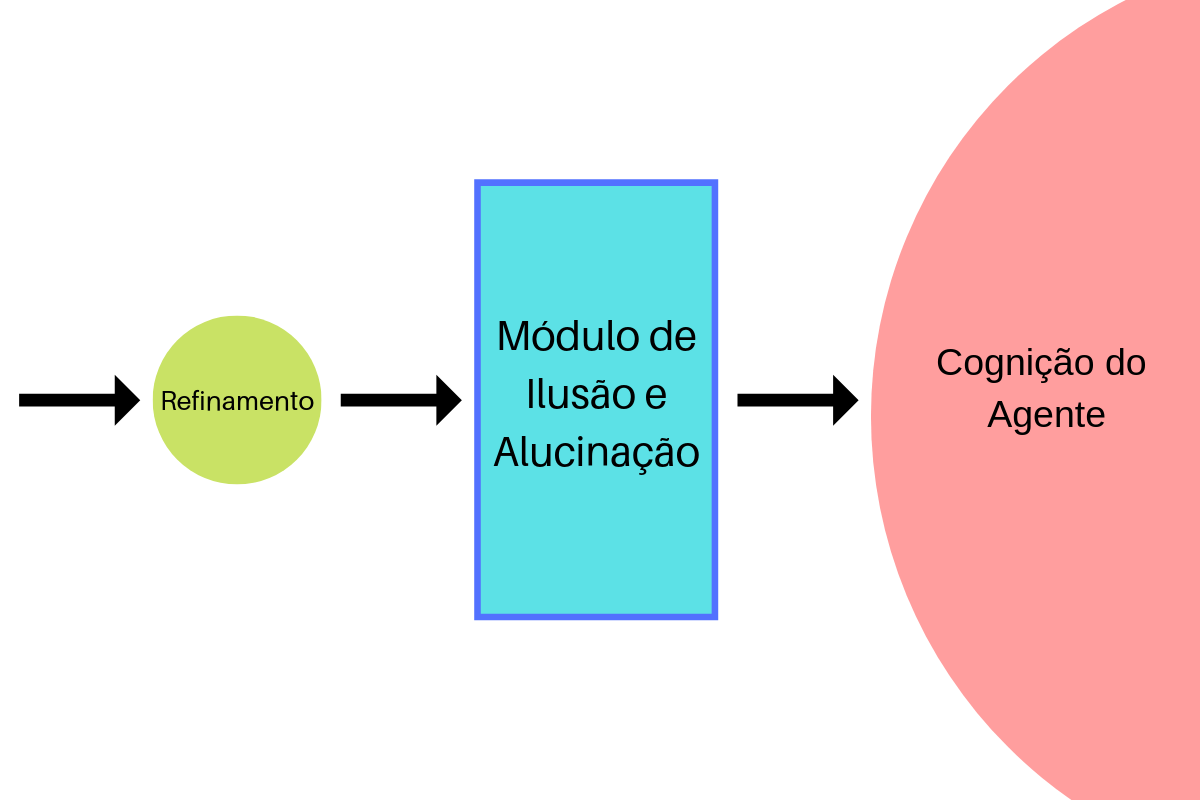
\includegraphics[width=0.8\textwidth]{Images/img2.png}
    \caption{Modelo de revisão de percepções.}
    \label{fig:method}
\end{figure}

\section{Módulo de refinamento}

O módulo de refinamento serve como uma primeira filtro para que percepções indesejadas pelo agente não cheguem até seu ciclo de raciocínio. O processo de refinamento é descrito pela definição \ref{def:refinamento}.

Caso não seja de interesse de uma determina arquitetura ou implementação de uma arquitetura refinar suas percepções, como pode ser o caso de um sistema especialista, o módulo de percepção pode simplesmente ter uma função tal que $f(x) = x$, com as percepções passando por dentro sem nenhum processo, possuindo assim o subconjunto próprio $\rho = p$.

\begin{example}
    Continuando o exemplo \ref{example::robo2}, as estrelas não fazem parte da área de atuação desse robô, e portanto para otimizarmos o processo de empacotamento é possível utilizar o módulo de percepções para refinar a informação recebida pelos sensores para enviar menos informações desnecessárias para a cognição do agente. Nesse exemplo, o robô pode ser implementado com uma função $\theta$ que realiza percepção ativa, removendo assim as percepções que não fazem sentido dentro do contexto em que ele está inserido. O conjunto de percepções $p$ passa pelo processo de percepção ativa e devolve $\rho$, que tem nesse caso específico, sendo $s$ o conjunto de percepções possíveis envolvendo estrelas, um comportamento tal que o conjunto $p$ sob a operação $\theta$ retorna $\rho = p \cap \overline{s}$. 
    Para tornar o processo mais tangível, vamos supor que o agente recebe o conjunto $p_i$ de percepções, composto por $\{circle(stripped), triangle(smooth), star(yellow)\}$. A operação $\theta$ vai remover de $p_i$ os elementos contidos no conjunto $s$ de possíveis percepções envolvendo estrelas, conforme foi descrito anteriormente. Portanto, a saída do bloco de percepções será $\rho = \{cicle(stripped), triangle(smooth)\}$.
    
\end{example}{}

\section{Módulo de Alucinação e Ilusão}

\begin{figure}[h]
    \centering
    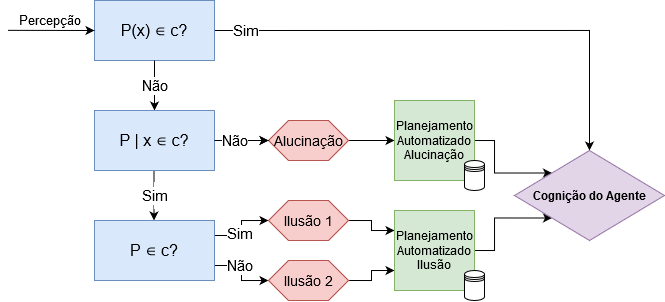
\includegraphics[width=0.8\textwidth]{Images/diagrama-modelo.png}
    \caption{Módulo de alucinação e ilusão.}
    \label{fig:model}
\end{figure}
 
 A figura \ref{fig:model} é a representação gráfica do módulo de alucinação e ilusão, que começa com a entrada $\rho$ sendo dirigida para o decisor 1. O primeiro decisor responde a pergunta: ``A percepção recebida está no código do agente?''. Caso a resposta for sim, consideramos a percepção como válida, e ela é enviada para a cognição do agente. Caso a resposta seja não, consideramos $\rho(x)$ uma anomalia, e enviamos ela para o segundo decisor, que responde a pergunta: ``O corpo ou o argumento do predicado $\rho(x)$ se encontra em alguma parte do código?''. Caso a resposta seja não, concluímos que a anomalia é uma alucinação. Caso contrário, ela é considerada uma ilusão e é enviada para o terceiro decisor. O terceiro decisor responde a pergunta: ``O corpo do predicado $\rho(x)$ está no código?''. Caso a resposta for sim, a ilusão é considerada uma ilusão classe 1, caso contrário, é considerado uma ilusão classe 2. Toda essa cadeia de decisores é representada pelo algoritmo abaixo:

\begin{algorithm}[H]
\SetKwInOut{Input}{input}
\Input{agent context \textit{c}, perception $\rho(x)$}

  \uIf{$\rho(x)$ is in \textit{c}}{
   $\rho(x)$ is a valid perception\;
   }\uElseIf{neither $\rho$ nor $x$ is in c}{
   $\rho(x)$ is a hallucination\;
   }\uElseIf{$\rho$ is in \texttt{c}}{
   $\rho(x)$ is an illusion class 1\;
  }\Else{$\rho(x)$ is an illusion class 2}
 \label{algorithm:decisor}
 \caption{Funcionamento dos decisores do módulo de ilusão e alucinação}
 \label{alg::selection}
\end{algorithm}

\begin{example}
    Para entender como as percepções são tratadas pelos decisores, vamos supor algumas entradas possíveis para o exemplo \ref{example::robo2}, que terão diferentes comportamentos ao longo do tempo de execução do nosso exemplo. Primeiro, vamos supor o caso mais básico, em que o agente recebe a percepção \texttt{quadrado(riscado)}. Essa é uma percepção completamente válida dentro do contexto do agente, pois ele possui um plano específico para tratar dessa percepção, que é empacotar o objeto com o papel vermelho. Portanto, nesse caso, $p(x) = \rho(x)$. Após sair do módulo de percepções, $\rho(x)$ passa como entrada para o decisor 1, que detecta que existe um plano específico para tratar da entrada, portanto a percepção é considerada válida e é diretamente enviada para a cognição do agente.

    Caso uma percepção não seja válida, ela é enviada para os decisores subsequentes, para que a anomalia seja devidamente classificada. 
\end{example}{}

\subsection{Bloco Avaliador}

Após a classificação da anomalia, ela é enviada para um bloco avaliador, que tratará de decidir qual anomalia pode ser considerada relevante para ocupar o planejamento automatizado e quais podem simplesmente retornar para o módulo de percepção para ajudar no processo de refinamento.
O funcionamento de um bloco avaliador deve permitir que alucinações ou ilusões seja processadas quando há tempo de processamento ocioso e o contexto permite. Para isso, vamos utilizar uma espécie de escalonador combinado com uma lista ponderada. Vamos considerar o tempo $c_m(\rho)$ o tempo médio de processamento gasto para cada percepção do conjunto $\rho$ recebido pelo agente, $a_m(\rho)$ o tempo médio do processamento das anomalias do conjunto $\rho$ recebida por um bloco de planejamento automatizado e $l_a$ a lista ponderada de $a$, onde $a$ é o índice que representa um dos três blocos avaliadores (de alucinação, ilusão classe 1 ou ilusão classe 2) utilizado para manter a generalidade. O principio do funcionamento da fila ponderada é o mesmo de uma fila comum, First in First Out (FIFO). Quando um elemento é inserido pela primeira vez na fila, ele recebe o peso 1. Quando uma cópia do mesmo elemento é inserida novamente, o elemento tem seu peso adicionado em 1, como mostra a figura \ref{filaPonderada}. Além disso, sendo $\rho$ o conjunto de percepções recebido pelo bloco de alucinação e ilusão, $|\rho|$ o número de percepções do conjunto e $\rho_a$ o número de anomalias.

O bloco avaliador seleciona quando uma percepção deve ser tratada através de uma função matemática, levando em conta o tempo médio de processamento de uma percepção válida e de uma anomalia, através da função de processamento. Além desse funcionamento básico, o bloco avaliador ainda contém um mecanismo para remover anomalias classificadas com irrelevantes para o sistema, através de uma função de limpeza. Caso essa função retorne verdadeiro, todos os elementos de peso 1 da sua respectiva lista são removidos. Essas duas funções serão trabalhadas na seção de formalismo.

\begin{figure}[h!]
    \centering
    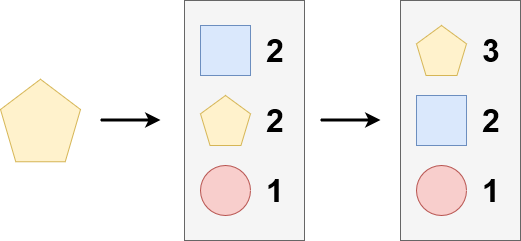
\includegraphics[width=0.49\textwidth]{Images/filaPonderada.png}
    \caption{Exemplo de fila ponderada.}
    \label{filaPonderada}
\end{figure}

\begin{example}
    Vamos supor que a percepção recebida pelo agente foi \texttt{lua(serrilhada)}. Lua não é um item que deveria ser percebido pelo agente, mas ou a implementação da percepção ativa foi simplória demais, simplesmente filtrando as estrelas, ou houve alguma falha que permitiu que ela chegasse ao módulo de alucinação e ilusão. Uma das propostas do modelo é detectar esse tipo de anomalia, que é uma falha completa do sistema. Quando ela chega ao decisor 1, é classificada como anomalia, pois não faz parte do escopo do agente. Em seguida, a percepção é enviada para o decisor 2, que verifica que não existe nenhuma menção de nenhuma parte da percepção no comportamento do robô, ou seja, é uma alucinação. Uma vez detectada a alucinação, a percepção segue para o bloco avaliador, onde será inserida na fila ponderada com o peso 1. Como consideramos apenas uma percepção recebida, e essa percepção é considerada uma anomalia, a equação da função de processamento é validada, e a anomalia segue para o bloco de planejamento automatizado.
\end{example}{}

\subsection{Bloco de Planejamento Automatizado}

O bloco de planejamento automatizado é potencialmente a parte mais custosa computacionalmente, e a parte mais difícil de ser implementada por todo o sistema. Um planejamento automatizado puramente simbólico tende a ser extremamente pesado, uma vez que pode considerar milhares de alternativas para o estado de mundo atual, tentando chegar mais perto de seu objetivo. Um processo de planejamento automatizado conexionista é uma opção, já que estamos tratando de uma análise incompleta do mundo, tratando do desconhecido. Teorias mais rebuscadas como criatividade computacional\cite{colton2012computational} podem ser adicionadas aqui, criando mais uma camada de complexidade para o agente, mas em troca dando um resultado ainda mais preciso para a avaliação da qualidade da percepção.

Uma percepção pode chegar ao bloco de planejamento automatizado quando ela for a primeira na fila ponderada e a função de processamento retornar verdadeiro. De um ciclo para outro, as percepções permanecem na fila, a não ser que sejam descartadas pelo mecanismo de limpeza. Nosso modelo não explicita qual é a ordem que os blocos avaliadores devem processar suas filas para mandar anomalias para o planejamento automatizado, ficando a cargo da implementação em questão tomar essa decisão.


\begin{example}
    Para mostrar o caminho que faz uma ilusão, vamos considerar que o agente recebe em duas esteiras a percepção \texttt{triangulo(listrado)}. Não existem triângulos listrados na loja, mas como $\theta$ não filtra essa percepção, ela vai chegar ao decisor 1. Como não existe um plano específico para tratar essa percepção, ela é considerada uma anomalia, e é encaminhada ao decisor 2. Como existe um plano para tratar de triângulos lisos, a percepção é então classificada como uma ilusão, e vai para o terceiro decisor. Nele, como o plano trata triângulos, a percepção é considerada uma ilusão classe 1. Finalmente após a percepção ter sido classificada corretamente, ela é enviada para o bloco avaliador, e é inserida na fila ponderada com peso 1. Depois disso, a percepção da segunda esteira, que é igual a que já foi tratada, chega ao bloco de alucinação e ilusão. Essa percepção vai fazer o mesmo caminho até o bloco avaliador e o peso da anomalia já presente na fila é aumentada para 2. Como duas percepções foram consideradas anomalias, vamos considerar que a função de processamento seja satisfeita, e o bloco avaliador passa essa anomalia para o bloco de planejamento automatizado.
    
    Após uma percepção ser considerada relevante para ser enviada ao planejamento automatizado, ela deve gerar um novo plano para aquela percepção a ser adicionada ao conjunto de planos do agente, e essa percepção então deixará de ser uma anomalia. Ilusões e alucinações tem blocos de planejamento automatizado separados para permitir que duas implementações completamente diferentes sejam utilizadas de acordo com a função do agente e a necessidade de criar novos planos eficientes. Retomando o exemplo dois, quando o planejamento automatizado de alucinações recebe a percepção \texttt{lua(serrilhada)}, um processo de planejamento automatizado deve ser executado. Para esse exemplo, consideremos um planejamento automatizado puramente simbólico, que analisa uma grande quantidade de estados futuros possíveis para o ambiente em que o robô está inserido e seleciona aquele que será mais eficiente para que o agente se aproxime de seu objetivo principal (terminar de empacotar os itens). Isso é extremamente custoso, mas como alucinações são muito raras para esse agente em questão, pois ele já tenta eliminar ao máximo percepções fora de seu escopo através da percepção ativa. Portanto, é um custo que vale a pena pois vai gerar um plano eficiente, evitando novas alucinações. No exemplo, é possível que a lua seja resultado de um corte errado na peça circular. Portanto, o agente precisa descartar esse item, para evitar gasto com embalagem desnecessária e que o item seja repassada para uma próxima etapa, gerando ainda mais custo. Assim, um novo plano da forma \texttt{lua(serrilhada) -> descartar} é adicionado, e \texttt{lua(serrilhada)} deixa de ser uma alucinação.

    No caso da percepção \texttt{triângulo(listrado)} do segundo exemplo, o agente poderia ter um bloco de planejamento automatizado baseado em uma rede baysiana, uma vez que ilusões podem ser muito mais comuns e o agente já tem uma breve noção do que deve ser feita com objetos do tipo. \texttt{triângulo(listrado)} pode ser um novo item a venda na loja, e como já foi verificado em duas esteiras diferentes, faz sentido que ele não seja uma mera falha de sensores. Assim, o planejamento automatizado pode inferir o plano \texttt{triângulo(listrado) -> empacotar}, permitindo que o agente tenha um aprendizado dinâmico resultado da adição de um novo plano em seu conjunto de planos. Assim como no caso da ilusão, uma vez que esse plano novo foi adicionado a percepção original deixa de ser uma anomalia, uma vez que faz parte do contexto em que o agente está trabalhando.

\end{example}{}

\section{Formalização}

A formalização foi realizada em um modelo de cascata, onde se começa com uma única tupla, que se desdobra para conceitos mais complexos e específicos. O objetivo disso é criar camadas de abstração, sobre as quais podem ser criadas variações de acordo com a necessidade de implementações específicas ou da integração com arquiteturas cognitivas.

 O bloco básico do modelo proposto, chamado de \emph{Modelo de Revisão de Percepções}, é composto por duas unidades: (i) um módulo para alucinação e ilusão $M_{ih}$; (ii) uma função de refinamento $\theta$. O módulo de ilusão e alucinação é uma quádrupla, apresentada na definição \ref{def:illuHallu}. A função de refinamento é uma função abstrata, cuja entrada é obtida através dos sensores do agentes e a saída é a entrada do módulo de alucinação e ilusão. Ela recebe um conjunto de percepções qualquer $p$ e retorna um subconjunto próprio $\rho$, ou seja, é uma função que pode ou não reduzir o número de percepções que são enviadas ao modulo de ilusão e alucinação.

\begin{definition}{}
    Um modelo de revisão de percepções é uma dupla $R = \langle M_{ih}, \theta \rangle$, onde:
    
    \begin{itemize}
        \item $M_{ih}$ é o bloco de ilusão e alucinação; e
        \item $\theta$ é a função de refinamento $\theta(p) = \rho$, onde $p$ é um conjunto de percepções e $\rho$ é um subconjunto próprio de $p$.
    \end{itemize}{}
    
\end{definition}

Após ter passado pela função $\theta$, as percepções $\rho$ irão passar pelo algoritmo \ref{alg::selection}, descrito por uma quádrupla, com conjuntos de decisores e blocos e uma função de transição.

\begin{definition}
\label{def:illuHallu}
    O bloco de alucinação e ilusão é uma quádrupla $M_{ih} = \langle D, Ab, Ap, \Delta \rangle$, onde:
    
    \begin{itemize}
        \item $D$ é o conjunto de decisores $D = \{d_{a}, d_{h}, d_{i}\}$, onde:
             \begin{itemize}
                \item $d_{a}$ é o decisor de anomalias, descrito pela função:
                \[ d_{a} = \left\{ \begin{array}{ll}
                0 & \mbox{se $\rho(x)$ está em $c$ \footnotemark};\\
                1 & \mbox{se $\rho(x)$ não está em $c$}.\end{array} \right. \]
             
                \item $d_{h}$ é o decisor de alucinação, descrito pela função:
                \[ d_{h} = \left\{ \begin{array}{ll}
                0 & \mbox{se nem $\rho$ nem $(x)$ está em $c$};\\
                1 & \mbox{se $\rho$ ou $(x)$ está em $c$}.\end{array} \right. \]
                
                \item $d_{i}$ é o decisor de ilusão, definido pela função:
                \[ d_{i} = \left\{ \begin{array}{ll}
                0 & \mbox{se $\rho$ está em $c$};\\
                1 & \mbox{se $(x)$ está em $c$}.\end{array} \right. \]
            \end{itemize}
        
        \footnotetext{ $c$ é o contexto do agente, de acordo com a definição \ref{definition::context}.}
        
        \item $Ab$ é o conjunto de blocos avaliadores $Ab = \{Ab_{h}, Ab_{i1}, Ab_{i2}\}$, onde $Ab_{h}$ é o bloco de avaliação de alucinações, $Ab_{i1}$ é o bloco de avaliação de ilusões classe 1 e $Ab_{i2}$ é o bloco de avaliação de ilusões classe 2.
        
        \item $Ap$ é o conjunto de blocos de planejamento automatizado $Ap = \{Ap_{h}, Ap_{i}\}$, onde $Ap_{h}$ é o bloco de planejamento automatizado de alucinações e $Ap_{i}$ é o bloco de planejamento automatizado de ilusões.
        
        \item $\Delta$ é a função de transição definido pela tabela abaixo, onde $out$ é um estado final, que leva a percepção para fora do modelo de revisão de percepções, ou seja, pode ser tanto uma transição para descartar a percepção quanto para levá-la para o ciclo de raciocínio do agente como uma percepção válida.
        
            \begin{table}[htb]
                \centering
                \begin{tabular}{c c c c} 
                    \toprule
                    \textbf{State} & \textbf{0} & \textbf{1} \\
                    \midrule
                    $d_{a}$     & $out$     & $d_{h}$       \\
                    $d_{h}$     & $Ab_{h}$  & $d_{i}$       \\
                    $d_{i}$     & $Ab_{i1}$ & $Ab_{i2}$     \\
                    $Ab_{h}$    & $out$     & $Ap_{h}$      \\
                    $Ab_{i1}$   & $out$     & $Ap_{i}$      \\
                    $Ab_{i2}$   & $out$     & $Ap_{i}$      \\
                    \bottomrule
                \end{tabular}
                \label{transition-table}
                \caption{Tabela de transição $\Delta$ do módulo de ilusão e alucinação}
                
            \end{table}
    \end{itemize}{}
\end{definition}{}

O módulo de alucinação e ilusão é o corpo principal do modelo. Ele recebe uma entrada $\rho$, que é a saída da função de refinamento apresentada na definição 1, e processa cada um dos elementos $\rho(x)$ desse conjunto, através de decisores e blocos de avaliação, percorrendo o modelo de acordo com as transições descritas pela função de transição $\Delta$. Os três decisores do conjunto $D$ fazem a triagem para detectar se a percepção $\rho(x)$ é uma anomalia, e que tipo de anomalia é. Após passar pelos três decisores, saberemos se essa percepção é valida, é uma alucinação, é uma ilusão tipo 1 ou uma ilusão tipo 2.

Após ter passado pelos decisores, a percepção fica armazenada nos blocos avaliadores, que serão descritos posteriormente, onde por fim poderá ser descartada ou enviada para um módulo de planejamento automatizado.

\begin{definition}
    Um bloco avaliador é uma tripla $Ab_{x} = \langle L, Pf, Cf) \rangle$, $x \in \{h, i1, i2\}$, onde:

    \begin{itemize}
        \item $L$ é uma lista ordenada pelo número de vezes que uma mesma anomalia é dada como entrada;
        \item $Pf$ é a função de processamento, definida abaixo:
            
             \[ Pf = \left\{ \begin{array}{ll}
                        1 & \mbox{if $T_{m}(A) \leq T_{m}(V) * (|A| - |A_{pr}|)$;}\\
                        0 & \mbox{caso contrário}.\end{array} \right. \]
        
            
            Onde:
            
            \begin{itemize}
                \item $T_{m}$ é a função que retorna a média do tempo gasto para processar as percepções de um conjunto;
                \item $A$ é o conjunto de anomalias, $A(x)$ é um elemento específico $x$ e $|A|$ o número de anomalias do conjunto;
                \item $A_{pr}$ é o conjunto de anomalias que já foram validades para serem processadas pela função de processamento neste ciclo de raciocínio ($A_{pr}$ é instanciada vazia a cada ciclo de raciocínio), e $|A_{pr}|$ o número de anomalias desse conjunto.
                \item $V$ é o conjunto de percepções válidas.
            \end{itemize}{}
        
        \item $Cf$ é a função de limpeza conforme definida abaixo, sendo $\alpha$ um coeficiente variável que precisa ser definido pela instância do modelo de revisão de percepções:
        
        \[ Cf = \left\{ \begin{array}{ll}
                        1 & \mbox{se  $Ce = Verdadeiro$;}\\
                        0 & \mbox{caso contrário}.\end{array} \right. \]
            
            \[ Ce = \sum_{i=1}^{|L|} P_{n}(L_{i}) > \alpha \sum_{j=1}^{|L|} P_{1}(L_{j}) \]
            
            Onde:
            
            \begin{itemize}
                \item $L$ é a lista ordenada do bloco, sendo $|L|$ o número de anomalias únicas e $L_{i}$ a anomalia $i$ da lista.
                \item $P$ é a função $P(L_{i}) = |L_{i}|$, sendo $|L_{i}|$ o peso da anomalia especificada (número de entradas recebidas dessa mesma anomalia na lista). A função $P$ é utilizada para especificar as seguintes funções:
                \\
                
                    (i) $ P_{1}(L_{i}) = \left\{ \begin{array}{ll}
                        1 & \mbox{se $P(L_{i}) = 1$;}\\
                        0 & \mbox{caso contrário}.\end{array} \right. $
                \\
                
                    (ii) $ P_{n}(L_{i}) = \left\{ \begin{array}{ll}
                        P(L{i}) & \mbox{se $P(L_{i}) > 1$;}\\
                        0 & \mbox{caso contrário}.\end{array} \right. $
            \end{itemize}{}
    \end{itemize}
\end{definition}{}

A terceira definição é a de bloco de avaliação ($Ab$). Um $Ab$ é um módulo do modelo que é responsável por armazenar as anomalias detectadas e decidir se elas serão processadas pelo agente ou não. É descrito por uma tripla, constituída por uma lista ordenada $L$, uma função de processamento $Pf$ e uma função de limpeza $Cf$. $L$ é uma lista organizada pela recorrência de elementos inseridos nela, onde cada elemento só aparece uma vez e contém um número de vezes que o mesmo elemento já foi inserido nela, chamado de peso. Nesse modelo, os elementos são as anomalias percebidas pelo agente, e o peso é o número de vezes que o agente percebeu a anomalia.

$Pf$ é uma função que avalia se uma anomalia será processada nesse ciclo de raciocínio ou se será armazenada para ser processada no futuro. Para isso, ela precisa de uma função que retorne o tempo médio previsto para o processamento de uma percepção $T_m$, seja ela uma percepção válida ou uma anomalia. Com base nessa função, $Pf$ retorna 1 caso o tempo médio de processamento de uma anomalia seja menor que o tempo médio de processamento de uma percepção válida multiplicado pelo número de anomalias que fazem parte desse ciclo de raciocínio menos o número de anomalias que já foram aprovadas pelo bloco avaliador, e zero caso contrário.

De maneira simplificada, o que essa função busca evitar que o modelo de revisão de percepção gaste mais tempo de processamento do que ele gastaria caso não estivesse sendo utilizado, processando apenas as anomalias que aparecem de maneira mais recorrente para o agente.

$Cf$ é uma função que realiza a limpeza de $L$. Conforme os ciclos de raciocínio forem passando, $L$ tende a possuir diversas anomalias que foram percebidas apenas uma única vez. Dessa maneira, uma grande quantidade de memória seria necessária para armazenar as possíveis centenas de anomalias que podem nunca ser processadas. Assim, a função $Cf$ verifica se a equação $Ce$ é verdadeira ou falsa. Ela é verdadeira quando o número de anomalias que apareceram uma única vez é maior que a soma dos pesos das anomalias que apareceram mais de uma vez (o peso é o número atrelado a cada anomalia, que representa quantas vezes elas já foram inseridas na linha). Quando a função for verdadeira, o bloco avaliador remove todas as anomalias de peso 1 da lista.

\begin{definition}
    Um bloco de planejamento automatizado é uma instância do modelo conceitual de planejamento automatizado (definição \ref{definition::autoplanning}).
\end{definition}
% \chapter{Simulação e Resultados}
\chapter{Experimentos}

Para este trabalho foram realizados três experimentos com o objetivo de averiguar se o modelo HAIL é funcional ou não. Esses experimentos não possuem um domínio específico, ou seja, não há um ambiente real onde o agente está inserido, ele recebe percepções aleatórias geradas pelo simulador e os planos inicias do agente não são relevantes para os testes.

Os dois primeiros experimentos foram implementados utilizando o design $2^k$ fatorial \cite{jain1990art}. Esse tipo de design consiste em variar $k$ fatores em 2 níveis diferentes, -1 e 1, que são extremos opostos. Por exemplo, em uma pesquisa ligada a um processador, um fator pode ser o número de núcleos, e seus níveis serem 1 núcleo e 8 núcleos. O fator é uma variável livre, utilizada para analisar a variação de uma variável dependente qualquer. Os fatores e as variáveis livres utilizadas estão nas Tabelas \ref{table:experiments_factors} e \ref{table:experiments_variables}, respectivamente. A análise do impacto dos fatores foi realizada utilizando a equação de regressão não linear do design $2^k$ fatorial.
%O código implementado para essa análise está disponível no anexo [NÚMERO].

\begin{table}[h!]
    \begin{center}
        \caption{ Fatores utilizados nos experimentos realizados com o modelo HAIL. }
        \label{table:experiments_factors}
        \begin{tabular}{|c|c|c|c|}
        \hline
        \textbf{Fatores} & \textbf{Sigla} & \textbf{Nível -1} & \textbf{Nível 1} \\
        \hline
        Porcentagem de Percepções Inválidas & PPI & 5\% & 95\%  \\
        \hline
        Tempo Médio gasto pelo planejamento Automatizado & TMA & 1/2 T & 64 T \\
        \hline
        Tempo Médio gasto em um Ciclo de raciocínio & TMC & 01 T & 32 T \\
        \hline
        Número de Percepções recebidas por Ciclo & NPC & 01 & 16 \\
        \hline
    \end{tabular}{}
    \legend{Fonte: Autor.}
    \end{center}
\end{table}{}

\begin{table}[h!]
    \begin{center}
        \caption{ Variáveis dependentes analisadas nos experimentos realizados com o modelo HAIL. }
        \label{table:experiments_variables}
        \begin{tabularx}{\textwidth}{ |Y|Y| }
            \hline
            \textbf{Variáveis} & \textbf{Motivação} \\
            \hline
            Tempo Virtual Decorrido & Medir desempenho geral do modelo \\
            \hline
            Planos Criados & Avaliar potencial do modelo de inserir aprendizado em arquiteturas que não o possuem \\
            \hline
            Percepções Válidas Processadas & Analisar a capacidade do modelo de ganhar desempenho ao longo do tempo\\
            \hline
        \end{tabularx}{}
    \legend{Fonte: Autor.}
    \end{center}{}
\end{table}

O terceiro experimento não utiliza o design $2^k$ fatorial. Após as simulações do segundo experimento, foi identificada a demanda de analisar como o HAIL era impactado com o processo contínuo de aprendizado fornecido pelo bloco de planejamento automatizado. Este experimento não utiliza um design específico, e será melhor explicado na Seção \ref{section:exp3}.

Os experimentos consistem em diversas simulações, que submetem o modelo proposto ao processo de revisão de um grande número de percepções. Uma simulação possui 5000 ciclos de percepção, sendo que cada ciclo pode possuir uma ou várias percepções. Essas percepções podem ser válidas (pertencentes ao contexto do agente) ou inválidas (não pertencentes ao contexto do agente), sendo que a proporção entre o tipo de percepções é definido pela PPI. As percepções são produzidas aleatoriamente por um gerador de percepções. 

O gerador de percepções cria as percepções válidas sorteando símbolos que pertencem ao contexto do agente, e as percepções inválidas são criadas utilizando o pacote \texttt{RandomWords} \cite{pipRandomWords2}, que gera palavras em inglês aleatórias. As percepções são símbolos compostos da forma \texttt{corpo(argumento)}, e a quantidade de percepções válidas e inválidas geradas é baseado no PPI e TMA da simulação executada.

Cada ciclo da simulação segue os seguintes passos:

\begin{enumerate}
    \item Gerar as percepções da simulação;
    \item Iterar sobre cada um dos ciclos, passando as percepções para o modelo implementado;
    \item Salvar os resultados, o agente final (com novos planos gerados pelo módulo de planejamento automatizado) e as percepções de cada ciclo em arquivos CSV.
\end{enumerate}

\begin{figure}[h!]
    \centering
    \caption{Diagrama da execução de uma iteração de cada simulação.}
    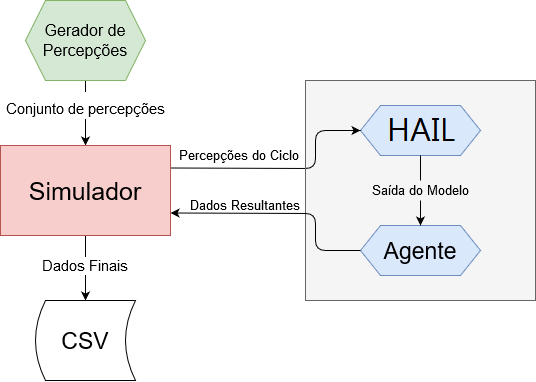
\includegraphics[width=0.8\textwidth]{images/diagrama-simulacao.png}
    \legend{Fonte: Autor.}
    \label{fig:diagrama-simulacao}
\end{figure}

Além da configuração dos valores dos fatores, é possível configurar se um agente será recarregado (ou seja, se ele deve manter os planos gerados por uma simulação anterior) e se o simulador deve gerar novas percepções ou não, pulando a etapa 1 de cada ciclo.

Para mensurar o tempo gasto pelos processos do agente, será considerada uma unidade de tempo genérica T, e iremos considerar o tempo virtual da execução das simulações com base nessa unidade. Portanto em uma simulação que possui TMC de 1T e TMA de 64T, o tempo médio do planejamento automatizado é 64 vezes maior do que o tempo médio do ciclo de raciocínio do agente.

Foi utilizado o agente do Exemplo \ref{example::robo} nas simulações, mas ele não foi descrito de acordo com nenhuma linguagem de programação de agentes real. Suas regras utilizam o formato de notação $percepcao -> acao1; acao2; ...; acaoN$. As ações desta implementação, assim como as percepções, são símbolos da forma \texttt{corpo(argumento)}. O módulo de refinamento não foi implementado, ou seja, sua entrada e saída são equivalentes.

\section{Implementação}

A implementação do simulador foi feita em Python 3.7, e conta com três classes principais: \texttt{PerceptionGenerator}, \texttt{PerceptionRevision} e \texttt{Simulator}. As interações das classes do simulador a partir do método \texttt{main} estão ilustradas na Figura \ref{fig:diagrama-implementacao}.

\begin{figure}
    \centering
    \caption{Diagrama demonstrando o relacionamento entre as classes do simulador.}
    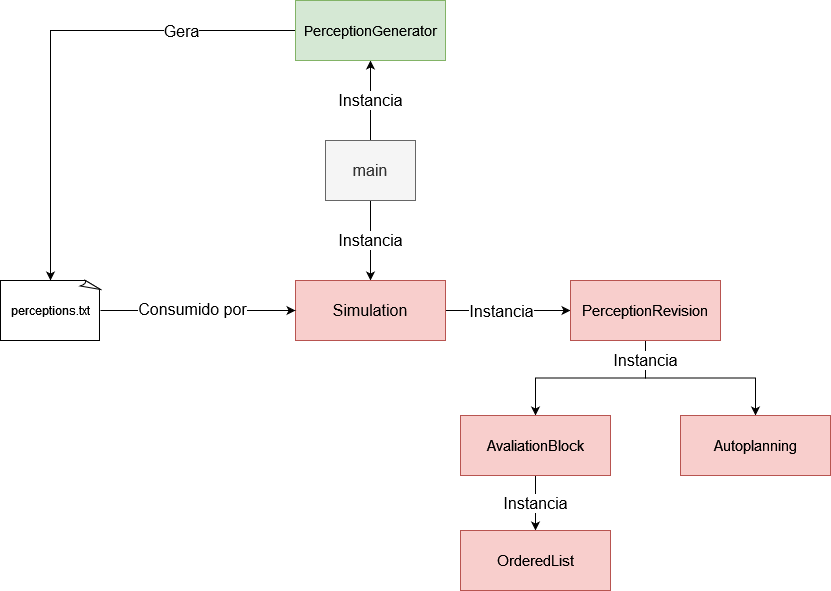
\includegraphics[width=\textwidth]{images/diagrama-implementacao.png}
    \legend{Fonte: Autor.}
    \label{fig:diagrama-implementacao}
\end{figure}

O gerador de percepções foi abstraído em um pacote chamado de \texttt{generator}, e sua classe é implementada no arquivo \texttt{perceptions.py}. Esta classe deve ser instanciada passando como argumento o número de ciclos de percepção que serão utilizados na simulação, a porcentagem de percepções inválidas e o número de percepções por ciclo. Depois de instanciado, é possível utilizar o objeto para chamar a função \texttt{generate}, que utiliza a configuração recebida para criar as percepções e escrevê-las num arquivo \texttt{perceptions.txt}. As percepções inválidas são geradas aleatoriamente com o pacote \texttt{RandomWords} e as percepções válidas são geradas a partir da especificação do arquivo \texttt{perceptions\_options.py}, onde são definidas o corpo e o argumento das percepções válidas.

O modelo HAIL foi implementado na classe \texttt{PerceptionRevision}, que está contido no arquivo \texttt{pr\_system.py}. Ele implementa cada um dos processos descritos no Capítulo \ref{chapter:model}. Quando esta classe é instanciada, ela primeiro extrai o contexto do agente através do método auxiliar \texttt{get\_agent\_context}, que percorre o arquivo do agente buscando os símbolos que compõem o contexto no corpo e no argumento dos símbolos dos planos. Depois disso, são instanciados os blocos de avaliação como atributos da classe do revisor, um para cada tipo de anomalia. Eles são implementados em uma classe chamada \texttt{AvaliationBlock}. Cada bloco guarda uma instância da classe \texttt{OrderedList}, que representa a lista ordenada definida pelo modelo. Por último, o bloco de planejamento \texttt{Autoplanner} é instanciado.

Como o bloco de planejamento automatizado não é o foco do trabalho, e possui uma grande complexidade de implementação, foi criado uma versão que cria um plano novo juntando a anomalia recebida com um conjunto aleatório de ações que o agente possui. Além disso, nessa implementação alucinações e ilusões utilizam o mesmo método de planejamento automatizado, portanto apenas um bloco é instanciado.

A anomalia \texttt{studies(distortion)} submetida ao planejamento automatizado pode gerar a percepção \texttt{studies(distortion) -> wrap\_up(circle)}, por exemplo. A implementação do \texttt{Autoplanner} gera um número aleatório de ações por plano, podendo ser uma ou no máximo o número de ações que o agente possui (nesse caso dois). 

O revisor de percepções possui um método principal utilizado nas simulações chamado \texttt{process\_perceptions}, que recebe uma lista de percepções, submete cada percepção ao fluxo do HAIL e então retorna o tempo virtual decorrido e o número de percepções válidas processadas. Para isso, cada percepção é classificada pelos decisores do módulo de alucinação e ilusão e então adicionada ao bloco avaliador designado. Quando todas as percepções foram classificadas, o modelo escolhe se vai processar as ilusões ou alucinações primeiro. Nessa implementação, essa escolha é feita aleatoriamente. Os blocos avaliadores passam pelo processo de validação da função de processamento, e anomalias são enviadas para o planejamento automatizado enquanto a função retornar verdadeiro.

Por fim, a classe \texttt{Simulation} utiliza as duas classes descritas anteriormente para executar a simulação. As percepções do arquivo \texttt{perceptions.txt} são lidas pelo método \texttt{run}, executando cada um dos ciclos de percepção utilizando uma instância da classe \texttt{PerceptionRevision}. Os valores finais de tempo virtual, percepções processadas e planos criados são retornados e guardados em um arquivo CSV.

Além da simulação, outro projeto foi criado para analisar o impacto dos fatores, medir o erro dos experimentos e criar os gráficos. Ele também foi implementado em Python 3.7 e utiliza as ferramentas \texttt{pandas} \cite{reback2020pandas}, \texttt{matplotlib} \cite{Hunter:2007} e \texttt{seaborn} \cite{Waskom_seaborn_statistical_data_2021}.

\section{Experimento 1}

O objetivo do primeiro experimento é analisar o impacto da mudança dos fatores no desempenho do modelo através da analise da variação no tempo virtual decorrido e da quantidade de planos criados pelo módulo de planejamento automatizado. 

Esse experimento foi o primeiro realizado com a metodologia do  $2^k$ fatorial. Cada um dos fatores foi avaliado em ambos os níveis apresentados na Tabela \ref{table:experiments_factors}, resultando em dezesseis combinações diferentes, e portanto dezesseis simulações. O tempo virtual foi escolhido para termos uma métrica geral de desempenho do sistema, enquanto a quantidade de planos criadas foi escolhida por ser um dos principais diferenciais do sistema, e um de seus aspectos mais importantes.

Cada simulação foi repetida dez vezes, e a média dos resultados foi obtida. Isso foi feito para garantir que os valores obtidos não foram afetados pela geração aleatória de percepções. Quando repetições são adotadas no experimento normalmente utiliza-se a metodologia $2^k r$ fatorial, que leva em conta o erro obtido entre as diferentes execuções da simulação. Todavia, ao fazer a análise de erros o resíduo obtido foi descartável, com ordem de grandeza $e^{-12}$. Portanto, a metodologia de análise adotada foi a do  $2^k$ fatorial.

\subsection{Resultados}

As médias dos resultados de cada simulação estão apresentadas na Tabela \ref{table:experimento1}. O valor final do tempo virtual decorrido varia bastante, principalmente nas simulações com alto nível de percepções inválidas. Em dois momentos o tempo virtual foi 5000T. Esse valor exato se repetiu pois nessas simulações o TMC é 1, o TMA é 0.5 e o NPC é 16. Nessa configuração os ciclos de percepções válidas consumiam 1 unidade de tempo, totalizando um tempo virtual de 4750T. O bloco avaliado sempre permitia o processamento de 2 percepções inválidas (pois cada uma toma 0.5 unidades de tempo), e quase sempre há percepções inválidas disponíveis na fila pois entram 16 percepções inválidas por ciclo de percepções inválidas. Portanto, cada vez que o modelo processava percepções inválidas, ele consumia 1 unidade de tempo, e isso aconteceu 250 vezes (5\% de 5000).

\begin{table}[h!]
    \begin{center}
        \caption{ Resultados do experimento 1.}
        \label{table:experimento1}
        \begin{tabular}{ |c|c|c|c|c|c|c| }
            \hline
            \textbf{Simulação} & \textbf{PPI} & \textbf{TMC} & \textbf{TMA} & \textbf{NPC} & \textbf{Tempo Virtual} & \textbf{Planos Criados}\\
            \hline
            1 & 5\% & 1 & 1/2 & 1 & 4874.6T & 250.8\\
            \hline
            2 & 5\% & 1 & 1/2 & 16 & 5000.0T & 502.0\\
            \hline
            3 & 5\% & 1 & 64 & 1 & 20806.7T & 250.9\\
            \hline
            4 & 5\% & 1 & 64 & 16 & 20813.0T & 251.0\\
            \hline
            5 & 5\% & 32 & 1/2 & 1 & 152093.5T & 251.0\\
            \hline
            6 & 5\% & 32 & 1/2 & 16 & 153437.3T & 2932.2\\
            \hline
            7 & 5\% & 32 & 64 & 1 & 168028.8T & 250.9\\
            \hline
            8 & 5\% & 32 & 64 & 16 & 168032.0T & 251.0\\
            \hline
            9 & 95\% & 1 & 1/2 & 1 & 3229.2T & 3541.6\\
            \hline
            10 & 95\% & 1 & 1/2 & 16 & 5000.00T & 9303.8\\
            \hline
            11 & 95\% & 1 & 64 & 1 & 228668.9T & 3550.3\\
            \hline
            12 & 95\% & 1 & 64 & 16 & 304300.4T & 4750.8\\
            \hline
            13 & 95\% & 32 & 1/2 & 1 & 48521.5T & 3539.0\\
            \hline
            14 & 95\% & 32 & 1/2 & 16 & 140683.3T & 4073.8\\
            \hline
            15 & 95\% & 32 & 64 & 1 & 273609.6T & 3550.3\\
            \hline
            16 & 95\% & 32 & 64 & 16 & 312032.0T & 4751.0\\
            \hline
        \end{tabular}{}
    \legend{Fonte: Autor.}
    \end{center}{}
\end{table}

O número de planos criados se agruparam em certos conjuntos de valores, de acordo com os níveis dos fatores. Como esperado, as simulações com menor porcentagem de percepções inválidas criaram menos planos, pois houveram menos anomalias, logo menos material para o módulo de planejamento automatizado trabalhar. A Figura \ref{fig:pc_occurrences} mostra a ocorrência de valores próximos de planos criados para cada uma das faixas obtidas nas simulações. Por exemplo, as simulações 12 e 16 tiveram aproximadamente 4750 percepções criadas, portanto foram agrupadas na mesma faixa no gráfico. Essas faixas de valores indicam que há uma discrepância entre as simulações com PPI de 5\% (com 6 ocorrências de aproximadamente 250 planos criados) e as simulações com PPI 95\%. Com isso, é possível notar que a principal condição para que o bloco de planejamento automatizado crie uma quantidade elevada de planos novos é um grande percentual de anomalias em relação ao total de percepções recebidas.

\begin{figure}[h!]
    \centering
    \caption{Recorrência do valor final de Planos Criados nas simulações realizadas.}
    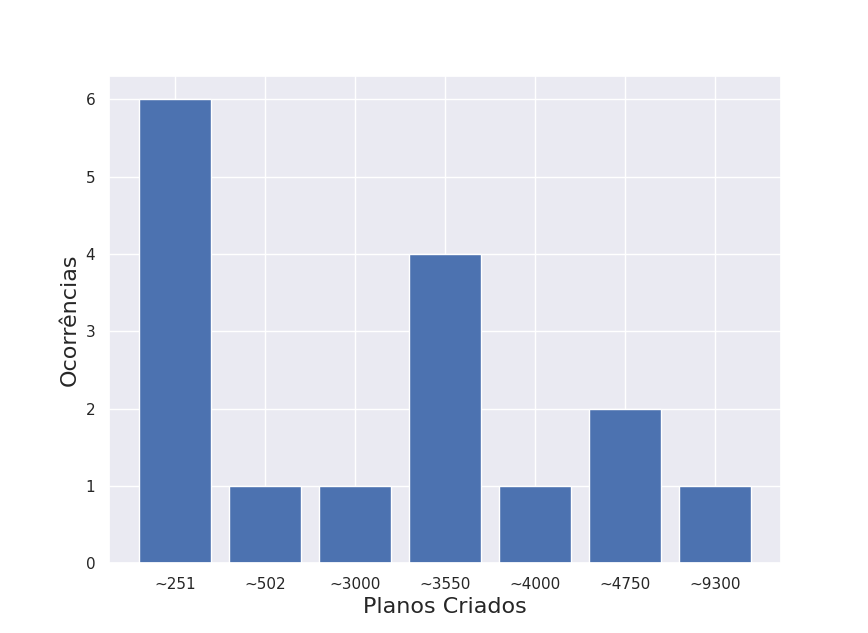
\includegraphics[width=1\textwidth]{images/plans_created_occurrences.png}
    \legend{Fonte: Autor.}
    \label{fig:pc_occurrences}
\end{figure}

\subsection{Análise de fatores}

Conforme mostra a Tabela \ref{tab:experimento1fatores}, na variável dependente de Tempo Virtual, os fatores TMC e TMA isolados tiveram uma alta porcentagem de impacto. Isso porque a contagem do tempo virtual acontece em função do tempo médio do ciclo de raciocínio e do tempo médio do planejamento automatizado. Portanto, a interferência nesses fatores influencia diretamente o resultado final. Além disso, a combinação dos fatores PPI + TMA teve um impacto de 24.13\%. Isoladamente, PPI e TMA possuem porcentagens altas (12.69 e 31.64, respectivamente) e quanto mais percepções inválidas há, maior o tempo gasto no planejamento automatizado, pois mais anomalias podem ser processadas. Como cada fator possui impacto alto e seus valores interferem diretamente um com o outro, a combinação de ambos acaba sendo relevante para o resultado das simulações. Por outro lado, TMC possui 22.20\% de impacto, mas a combinação PPI + TMC possui apenas 4.16, pois a porcentagem de percepções inválidas não interage diretamente com o tempo gasto no ciclo de raciocínio.

Isso demonstra como uma combinação de alta taxa de percepções inválidas com um tempo de planejamento automatizado alto podem ser impactantes no NPC. Portanto, em situações com um grande volume de percepções, implementações que possuem um bloco de planejamento automatizado que consome muito tempo para criar novos planos podem prejudicar o desempenho do agente caso ele seja muito sensível ao tempo.

\begin{table}
    \begin{center}
        \caption{Análise dos fatores do experimento 1.}
        \label{tab:experimento1fatores}
        \begin{tabular}{ |c|c|c| }
            \hline
            \textbf{Fator} & \textbf{Efeito Tempo Virtual} & \textbf{Efeito Planos Criados}\\  
            \hline
            PPI & 12.69\% & 66.10\%\\
            \hline
            TMC & 22.20\% & 0.50\%\\
            \hline
            TMA & 31.64\% & 2.95\%\\
            \hline
            NPC & 1.44\% & 8.67\%\\
            \hline
            PPI + TMC & 4.16\% & 3.76\%\\
            \hline
            PPI + TMA & 24.13\% & 0.05\%\\
            \hline
            PPI + NPC & 1.39\% & 2.13\%\\
            \hline
            TMC + TMA & 0.55\% & 0.50\%\\
            \hline
            TMC + NPC & 0.10\% & 0.50\%\\
            \hline
            TMA + NPC & 0.01\% & 2.99\%\\
            \hline
            PPI + TMC + TMA & 0.53\% & 3.76\%\\
            \hline
            PPI + TMC + NPC & 0.09\% & 3.75\%\\
            \hline
            PPI + TMA + NPC & 0.02\% & 0.06\%\\
            \hline
            TMC + TMA + NPC & 0.54\% & 0.50\%\\
            \hline
            PPI + TMC + TMA + NPC & 0.52\% & 3.76\%\\
            \hline
        \end{tabular}{}
    \legend{Fonte: Autor.}
    \end{center}{}
\end{table}


Na variável dependente Planos Criados, o fator que mais impactou o resultado foi o PPI. Isso era o esperado, pois quanto mais percepções inválidas o modelo recebe, mais planos podem ser criados. Os demais fatores tiveram impactos mais baixos. O NPC teve 8.67\% de influência pois simulações com mais percepções inválidas por ciclo preenchem a fila ponderada mais rápido, permitindo que o bloco avaliador sempre possua elementos na fila ponderada para enviar ao bloco de planejamento automatizado.

%%%%%%%%%%%%%%%%%%%%%%%%%%%%%%%%%%%%%%%%%%%%%%%%%%%%%%%%%%%%%%%%%%%%

\section{Experimento 2}

O segundo experimento foi realizado para analisar o ganho de performance de um agente ao utilizar os planos criados com o bloco de planejamento automatizado. Esse segundo experimento segue a metodologia do primeiro, porém foi realizado apenas uma iteração para cada configuração de fatores (ao invés das dez repetições). Após ser realizada uma simulação com uma configuração de fatores foi realizada uma nova simulação com a mesma configuração, mas usando o agente resultante da primeira. Assim, os planos criados pelo agente foram reaproveitados. Ao invés de analisar quais são os fatores que mais influenciam nas variáveis dependentes, comparamos os resultados dessas variáveis antes e depois da criação de novos planos. As variáveis dependentes analisadas foram novamente o tempo virtual decorrido e o número de planos criados.

% Como a segunda simulação sempre vai ter menos planos criados que a primeira (pois o agente já passou pelo processo de aprendizado), as variáveis dependentes analisadas foram o tempo virtual decorrido e o número de planos criados. Essa nova variável foi escolhida pois caso o TMC for alto, na segunda simulação o tempo virtual será maior, pois o agente aprendeu novos planos e portanto menos percepções serão anomalias. Todavia, o tempo virtual não é capaz de mensurar o aprendizado do agente. Como um dos principais objetivos do HAIL é fornecer aprendizado, a métrica de percepções processadas ajuda a medir a redução de anomalias na segunda simulação.

Esse experimento pode ter sua configuração de fatores separadas em dois grupos: (I) o tempo de processamento de um ciclo de raciocínio é menor do que o tempo do planejamento automatizado; (II) o tempo do planejamento automatizado é menor que o tempo de processamento de um ciclo de raciocínio. Essa separação pode ser feita pois quanto mais planos são criados, menos percepções inválidas serão recebidas pelo agente. Portanto, se o tempo de processamento de um ciclo for maior que o da geração de novos planos, o tempo virtual gasto total usando um agente que já aprendeu vários planos será maior. Isso é uma troca realizada pois agora essas novas percepções (que eram antes anomalias) estão sendo recebidas pelo agente e resultando na execução de um plano.

\subsection{Resultados}

Os resultados estão separados em tabelas por variável dependente e por grupo, como descrito anteriormente. As tabelas contém o índice da simulação, os níveis dos fatores, os resultados da primeira e da segunda iteração (R1 e R2, respectivamente) e a relação percentual (RP) entre os resultados, ou seja, a proporção de R2 em relação a R1, obtido através do cálculo $(R2 * 100) / R1$.

Em todas as tabelas, podem ser observadas um menor efeito na relação percentual nas simulações que utilizaram o nível $-1$ do fator PPI (5\% de percepções inválidas). Isso acontece pois o modelo possui menor impacto em ambientes de baixo volume de percepções inválidas, uma vez que o bloco de planejamento automatizado apenas cria novos planos quando há percepções inválidas na fila ponderada do bloco avaliador.

Na Tabela \ref{table:vtaltv1}, a média da relação percentual foi de 75.26\%, se destacando a simulação 5 com uma relação percentual de 4.77\%. Com o tempo de planejamento automatizado alto, tempo de processamento de um ciclo de raciocínio baixo e apenas uma percepção por ciclo, há um grande ganho de desempenho, conforme explicado anteriormente. Um comportamento similar (porém invertido) pode ser observado na Tabela \ref{table:vtaltv2}, cuja média da relação percentual foi de 136.33\%. Nessas simulações, o esperado era que o tempo virtual subisse conforme a quantidade de planos criados aumentasse, pois o tempo gasto no planejamento automatizado é menor que o tempo gasto no ciclo de raciocínio.

\begin{table}
    \begin{center}
        \caption{Alteração no valor de tempo virtual nas simulações do grupo I.}
        \label{table:vtaltv1}
        \begin{tabular}{ |c|c|c|c|c|c|c|c| }
            \hline
            \textbf{Simulação} & \textbf{PPI} & \textbf{TMC} & \textbf{TMA} & \textbf{NPC} & \textbf{R1} & \textbf{R2} & \textbf{RP}\\
            \hline
            1.1 & 5\% & 1 & 64 & 1 & 20750T & 20687T & 99.70\%\\
            \hline
            1.2 & 5\% & 1 & 64 & 16 & 20813T & 20750T & 99.70\%\\
            \hline
            1.3 & 5\% & 32 & 64 & 1 & 168032T & 167968T & 99.96\%\\
            \hline
            1.4 & 5\% & 32 & 64 & 16 & 168032T & 168000T & 99.98\%\\
            \hline
            1.5 & 95\% & 1 & 64 & 1 & 227579T & 10859T & 4.77\%\\
            \hline
            1.6 & 95\% & 1 & 64 & 16 & 304313T & 177998T & 58.49\%\\
            \hline
            1.7 & 95\% & 32 & 64 & 1 & 273536T & 162400T & 59.37\%\\
            \hline
            1.8 & 95\% & 32 & 64 & 16 & 312032T & 250048T & 80.14\%\\
            \hline
            
        \end{tabular}{}
    \legend{Fonte: Autor.}
    \end{center}{}
\end{table}

\begin{table}
    \begin{center}
        \caption{ Alteração no valor de tempo virtual nas simulações do grupo II. }
        \label{table:vtaltv2}
        \begin{tabular}{ |c|c|c|c|c|c|c|c| }
            \hline
            \textbf{Simulação} & \textbf{PPI} & \textbf{TMC} & \textbf{TMA} & \textbf{NPC} & \textbf{R1} & \textbf{R2} & \textbf{RP}\\
            \hline
            2.1 & 5\% & 1 & 1/2 & 1 & 4874.5T & 4876.5T & 100.04\%\\
            \hline
            2.2 & 5\% & 1 & 1/2 & 16 & 5000T & 5000T & 100\%\\
            \hline
            2.3 & 5\% & 32 & 1/2 & 1 & 152093.5T & 152219.5T & 100.08\%\\
            \hline
            2.4 & 5\% & 32 & 1/2 & 16 & 153435.5T & 152887T & 99.64\%\\
            \hline
            2.5 & 95\% & 1 & 1/2 & 1 & 3228.5T & 4955T & 153.48\%\\
            \hline
            2.6 & 95\% & 1 & 1/2 & 16 & 5000T & 4944T & 98.88\%\\
            \hline
            2.7 & 95\% & 32 & 1/2 & 1 & 48458.5T & 157385.5T & 324.78\%\\
            \hline
            2.8 & 95\% & 32 & 1/2 & 16 & 160000T & 140631T & 113.77\%\\
            \hline
            
        \end{tabular}{}
    \legend{Fonte: Autor.}
    \end{center}{}
\end{table}

A outra variável analisada foi o número de percepções válidas processadas. A média de cada configuração de fatores foi de 30563.0625 percepções, enquanto nas segundas simulações foi de 40599.75, totalizando um ganho aproximado de 32.84\% de desempenho. Ou seja, apesar do ganho de tempo virtual em algumas situações, um maior número de percepções foi processada e resultou na execução de um plano do agente.

As Tabelas \ref{table:plansaltv1} e \ref{table:plansaltv2} mostram a variação do ganho de planos criados entre as simulações. Ambas apresentam uma queda drástica nessa variável nas simulações com 95\% de percepções inválidas, pois foram nessas simulações que o modelo pode criar mais planos (pois o planejamento automatizado é utilizado mais vezes). As simulações 1.6 e 1.8 possuem um resultado acima das
simulações 1.5 e 1.7, apesar das quatro possuírem PPI de 95\%, pois possuem mais percepções (16 vezes mais por conta do NPC) e processam no máximo uma percepção inválida por ciclo (pois o TMA é maior que o TMC).
A Tabela \ref{table:plansaltv2} possui valores ainda menores na relação percentual pois muitas percepções inválidas são processadas por ciclo, em especial na simulação 2.8, onde nenhum plano novo foi criado na segunda simulação. Isso ocorreu pois o TMC é alto, o TMA é baixo e ela possui o maior número possível de percepções inválidas, resultando em um uso constante do planejamento automatizado.

\begin{table}
    \begin{center}
        \caption{ Alteração no valor de planos criados nas simulações do grupo I. }
        \label{table:plansaltv1}
        \begin{tabular}{ |c|c|c|c|c|c|c|c| }
            \hline
            \textbf{Simulação} & \textbf{PPI} & \textbf{TMC} & \textbf{TMA} & \textbf{NPC} & \textbf{R1} & \textbf{R2} & \textbf{RP}\\
            \hline
            1.1 & 5\% & 1 & 64 & 1 & 250.0 & 249.0 & 99.60\%\\
            \hline
            1.2 & 5\% & 1 & 64 & 16 & 251.0 & 250.0 & 99.60\%\\
            \hline
            1.3 & 5\% & 32 & 64 & 1 & 251.0 & 249.0 & 99.20\%\\
            \hline
            1.4 & 5\% & 32 & 64 & 16 & 251.0 & 250.0 & 99.60\%\\
            \hline
            1.5 & 95\% & 1 & 64 & 1 & 3533.0 & 93.0 & 2.63\%\\
            \hline
            1.6 & 95\% & 1 & 64 & 16 & 4751.0 & 2746.0 & 57.80\%\\
            \hline
            1.7 & 95\% & 32 & 64 & 1 & 3548.0 & 75.0 & 2.11\%\\
            \hline
            1.8 & 95\% & 32 & 64 & 16 & 4751.0 & 2814.0 & 59.23\%\\
            \hline
            
        \end{tabular}{}
    \legend{Fonte: Autor.}
    \end{center}{}
\end{table}


\begin{table}
    \begin{center}
        \caption{ Alteração no valor de planos criados nas simulações do grupo II. }
        \label{table:plansaltv2}
        \begin{tabular}{ |c|c|c|c|c|c|c|c| }
            \hline
            \textbf{Simulação} & \textbf{PPI} & \textbf{TMC} & \textbf{TMA} & \textbf{NPC} & \textbf{R1} & \textbf{R2} & \textbf{RP}\\
            \hline
            2.1 & 5\% & 1 & 1/2 & 1 & 251.0 & 247.0 & 98.41\%\\
            \hline
            2.2 & 5\% & 1 & 1/2 & 16 & 502.0 & 500.0 & 99.60\%\\
            \hline
            2.3 & 5\% & 32 & 1/2 & 1 & 251.0 & 247.0 & 98.41\%\\
            \hline
            2.4 & 5\% & 32 & 1/2 & 16 & 2935.0 & 878.0 & 29.91\%\\
            \hline
            2.5 & 95\% & 1 & 1/2 & 1 & 3543.0 & 90.0 & 2.54\%\\
            \hline
            2.6 & 95\% & 1 & 1/2 & 16 & 9312.0 & 260.0 & 2.79\%\\
            \hline
            2.7 & 95\% & 32 & 1/2 & 1 & 3541.0 & 83.0 & 2.34\%\\
            \hline
            2.8 & 95\% & 32 & 1/2 & 16 & 4078.0 & 0.0 & 0.0\%\\
            \hline
            
        \end{tabular}{}
    \legend{Fonte: Autor.}
    \end{center}{}
\end{table}

\section{Experimento 3}

\label{section:exp3}

O terceiro experimento foi executado para observar a capacidade de aprendizado do agente ao longo do tempo. Nele foram executadas 5 simulações com os mesmos fatores dos experimentos anteriores, mas com valores diferentes (como demonstra a Tabela \ref{table:experiment3factors}). Entre uma simulação e outra o agente não foi recarregado, ou seja, manteve o aprendizado das simulações anteriores.

\begin{table}[h!]
    \begin{center}
        \caption{ Valor dos fatores no experimento 3. }
        \label{table:experiment3factors}
        \begin{tabular}{ |c|c| }
            \hline
            \textbf{Fator} & \textbf{Valor}\\
            \hline
            PPI & 50\%\\
            \hline
            TMC & 16\\
            \hline
            TMA & 32\\
            \hline
            NPC & 8\\
            \hline
        \end{tabular}{}
    \legend{Fonte: Autor.}
    \end{center}{}
\end{table}

Os resultados estão expostos na Tabela \ref{table:experiment3results}, mostrando o comportamento dos três fatores observados. Enquanto os planos criados diminuem a cada simulação, pois menos percepções são inválidas (uma vez que o agente aprende com as simulações anteriores), a quantidade de percepções válidas processadas aumenta. Esse comportamento é demonstrado na Figura \ref{fig:perceptions_v_plans-experiment3}. Além disso, o tempo virtual cai na mesma proporção que os planos criados diminuem, uma vez que a criação de um plano é duas vezes mais custosa em tempo do que o processamento de uma percepção válida nesse experimento.

\begin{table}
    \begin{center}
        \caption{ Resultados obtidos no experimento 3. }
        \label{table:experiment3results}
        \begin{tabular}{ |c|c|c|c| }
            \hline
            \textbf{Simulação} & \textbf{Planos Criados} & \textbf{Percepções Válidas Processadas} & \textbf{Tempo Virtual}\\
            \hline
            1 & 2501 & 21788 & 120016T \\
            \hline
            2 & 2454 & 30558 & 119264T \\
            \hline
            3 & 946 & 38641 & 95136T \\
            \hline
            4 & 40 & 39959 & 80640T \\
            \hline
            5 & 0 & 40000 & 80000T \\
            \hline
        \end{tabular}{}
    \legend{Fonte: Autor.}
    \end{center}{}
\end{table}



\begin{figure}
    \centering
    \caption{Evolução das percepções válidas processadas e dos planos novos criados ao longo das simulações.}
    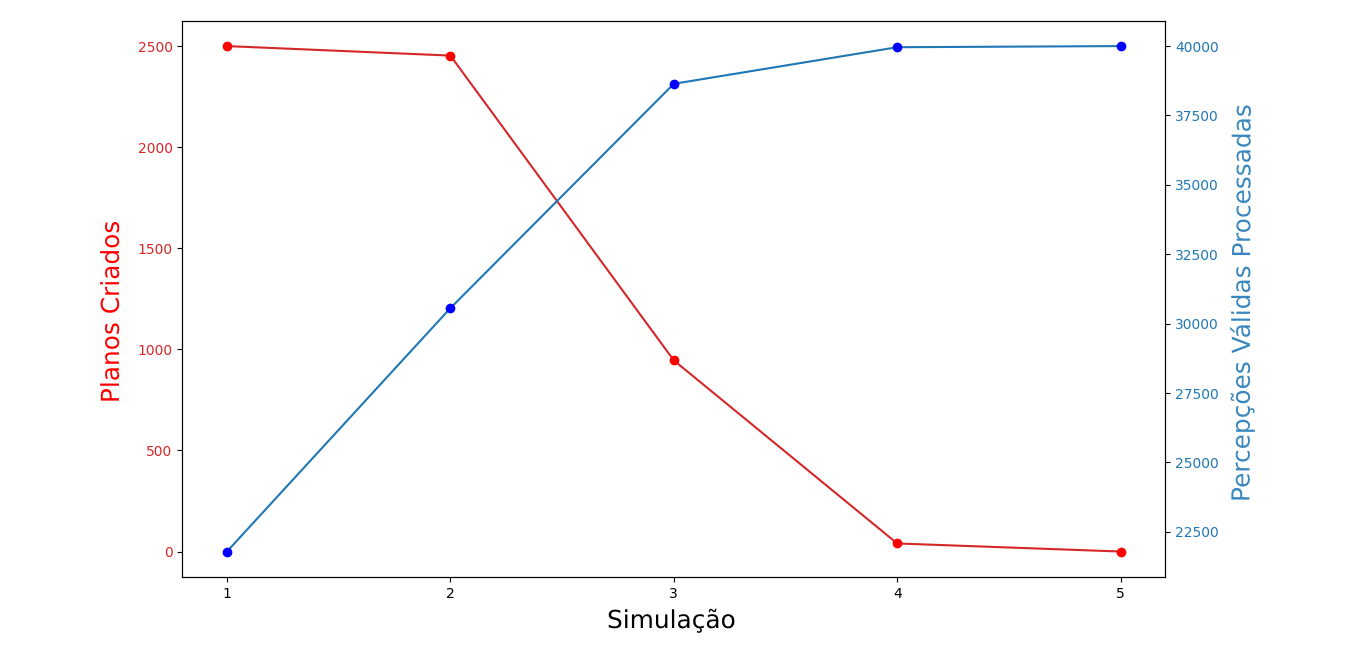
\includegraphics[width=\textwidth]{images/perceptions_vs_plans.png}
     \legend{Fonte: Autor.}
    \label{fig:perceptions_v_plans-experiment3}
\end{figure}

\section{Análise do modelo}

O principal objetivo dos experimentos era validar as ideias principais que compõem a proposta do modelo HAIL. Como as simulações foram realizadas sem ambiente e com um agente qualquer, os dados obtidos não podem ser usados como parâmetro de análise direta das qualidades do modelo, mas sim de seu funcionamento.

O primeiro experimento demonstrou que o módulo de ilusão e alucinação funciona como previsto: simulações com mais percepções inválidas e menor tempo médio de planejamento automatizado resultam em menos tempo virtual gasto e mais planos criados. Os grupos representados na Figura \ref{fig:pc_occurrences} demostram isso. As seis ocorrências do valor aproximado de 250 planos criados possuem PPI de 5\%. A única simulação com esse PPI que possui uma quantidade de planos criados aproximada aos valores das simulações com PPI 95\% possui TMA baixo e TMC e NPC altos, ou seja, muitos processos de planejamento automatizado são executados todos os ciclos, aumentando o número de planos criados. As demais simulações com esse PPI ou possuem poucas percepções por ciclo, ou o bloco avaliador não consegue enviar tantas anomalias para o planejamento automatizado devido aos valores de TMC e TMA.

Um dos objetivos do trabalho é criar um modelo capaz de aprender com as anomalias recebidas pelo agente através da percepção, e por isso o segundo e o terceiro experimentos abordam o mecanismo de aprendizado do HAIL. Com esses experimentos foi possível observar que o processo de seleção de anomalias que serão enviadas para o bloco de planejamento automatizado, desempenhado pelo bloco avaliador, é funcional.

O cenário ideal representado pelo experimento 3, onde todas as anomalias da primeira simulação se tornam parte do contexto do agente após poucas iterações, não tem como existir em uma situação real na qual a possibilidade de anomalias não é limitado por um gerador. Apesar disso, o experimento serve para demonstrar o funcionamento do módulo de ilusão e alucinação, pois os planos que são adicionados ao longo das simulações reduzem o tempo virtual e aumentam o número de percepções válidas processadas.

Com os resultados obtidos com os experimentos é possível afirmar que o modelo se comporta da maneira esperada, mas não é possível chegar a nenhuma conclusão relacionada à efetividade do modelo. Alguns cenários se mostraram favoráveis ao HAIL, como as simulações que possuem um grande volume de anomalias e baixo tempo de planejamento automatizado. Apesar disso, experimentos com cenários realistas e implementações acopladas a arquiteturas reais são necessários para validar que o modelo se comporta bem sob tais circunstâncias.
\chapter{Conclusão}

Neste trabalho, foi apresentado um modelo de revisão de percepções. Tal modelo, inspirado pelos conceitos de alucinação e ilusão, é capaz de reduzir as percepções recebidas, detectar percepções anômalas (que fogem do escopo de trabalho do agente), classificá-las de acordo com suas características como ilusão (do tipo 1 ou 2, conforme definido) ou alucinação e tratá-las, através do mecanismo de autoplanejamento.

O funcionamento do modelo foi descrito no capítulo 3, e sua formalização e implementação apresentadas no capítulo 4. Os experimentos realizados demonstram que o funcionamento do modelo é como esperado, sendo capaz de absorver as anomalias recebidas do ambiente e melhorar o comportamento do agente baseado nelas. Os resultados dos experimentos foram apresentados no capítulo 5. 
Analisando os resultados, é possível observar que o modelo funciona melhor em cenários onde há uma grande quantidade de percepções anômalas, possibilitando uma maior criação de planos novos. Além disso, o maior desafio do modelo é manter o desempenho do agente em cenários onde o tempo gasto pelo módulo de autoplanejamento é muito elevado.

Apesar dos experimentos terem resultados positivos, as simulações estavam limitadas a um cenário sem escopo, ou seja, sem objetivo no mundo real. Por conta disso, quase não haviam fatores aleatórios, tornando a análise extremamente precisa (com erros da ordem de grandeza de $e^{-12}$) mas também bastante limitada.
Portanto, é necessário ainda validar o modelo em mais três etapas: (i) acoplando-o a uma arquitetura cognitiva implementada, para verificar como ela se comporta em uma interação mais complexa com o ambiente; (ii) implementação de experimentos mais complexos, com simulações de alguma situação real que possa ter resultados mais palpáveis; (iii) a aplicação do modelo em agentes físicos, para verificar se ele é capaz de melhorar o desempenho de agentes em ambientes reais.




% ----------------------------------------------------------
% ELEMENTOS PÓS-TEXTUAIS
% ----------------------------------------------------------
\postextual
% ----------------------------------------------------------

% ----------------------------------------------------------
% Referências bibliográficas
% ----------------------------------------------------------
\begingroup
\printbibliography[title=REFERÊNCIAS]
\endgroup

% ----------------------------------------------------------
% Glossário
% ----------------------------------------------------------
%
% Consulte o manual da classe abntex2 para orientações sobre o glossário.
%
%\glossary

% ----------------------------------------------------------
% Apêndices
% ----------------------------------------------------------

% ---
% Inicia os apêndices
% ---
\begin{apendicesenv}
%	\partapendices*
	% ----------------------------------------------------------
\chapter{Código do simulador}
% ----------------------------------------------------------

O simulador foi implementado utilizando a versão 3.7 do Python, e o gerenciamento de pacotes foi feito com o Poetry. As dependências estão disponíveis no arquivo \texttt{pyproject.toml}.

\begin{section}{\_\_main\_\_.py}
    \begin{minted}
    [
    frame=lines,
    framesep=2mm,
    baselinestretch=1.2,
    breaklines=True,
    fontsize=\footnotesize,
    linenos
    ]
    {python}

from simulation import Simulation
from analyzer import get_mean
from generator.perceptions import PerceptionGenerator

import strings
from time import time
import pandas as pd
from shutil import copyfile
import click
import os

from proggy import BarInfo
from proggy.tty import TTYProgressBar


# Click was used in testing and first simulations, but was replaced with
# multiple function calls. This way, it is possible to run the program once
# for all 16 factors variation, instead of passing the arguments through console
# every time one simulation ends. Uncommenting this decorators and the first line
# from main enable console usage again.

# @click.command()
# @click.option("--generate", "-G", default=0, nargs=2, help=strings.generate_help)
# @click.option(
#     "--reload-agent/--not-reload", "-R/", default=True, help=strings.reload_help
# )
# @click.option("--reasoning-time", default=1.0, help=strings.reasoning_time_help)
# @click.option("--planning-time", default=32.0, help=strings.planning_time_help)
# @click.option(
#     "--perceptions-per-cycle", "-C", default=1, help=strings.perceptions_per_cycle_help
# )
# @click.option("--iterations", "-I", default=1, help=strings.iterations_help)
def run(
    generate,
    reload_agent,
    reasoning_time,
    planning_time,
    perceptions_per_cycle,
    iterations,
):

    start_time = time()
    vtimes = []
    pps = []
    pcs = []
    name_string = f"valid{generate[1]}reasoning{reasoning_time}planning{planning_time}" + "perceptions{perceptions_per_cycle}reload{str(reload_agent)}"

    with TTYProgressBar(BarInfo(size=30, total=iterations)) as p:

        for i in range(iterations):
            # print(f"-------------\nSIMULATION {i}\n-------------")

            if generate:
                g = PerceptionGenerator(*generate, perceptions_per_cycle)
                g.generate()
                if not os.path.exists(f'./data3/perceptions/{name_string}'):
                    os.makedirs(f'./data3/perceptions/{name_string}')
                copyfile("perceptions.txt", f"./data3/perceptions/{name_string}/iteration{i}.txt")

            s = Simulation(
                reasoning_time,
                planning_time,
                perceptions_per_cycle,
                reload_agent=reload_agent,
            )
            vtime, perceptions_processed, plans_created = s.start()
            vtimes.append(vtime)
            pps.append(perceptions_processed)
            pcs.append(plans_created)

            if not os.path.exists(f'./data3/agents/{name_string}'):
                    os.makedirs(f'./data3/agents/{name_string}')
            copyfile("agent.txt", f"./data3/agents/{name_string}/iteration{i}.txt")

            p.progress += 1

    final_time = time()
    total_time = final_time - start_time
    total_time = "{:.2f}".format(total_time)
    print(
        f"------------\nFinished Simulation\nTime elapsed: {total_time}s\n------------"
    )

    d = {"vtime": vtimes, "perceptions_processed": pps, "plans_created": pcs}
    df = pd.DataFrame(data=d)
    
    df.to_csv(f'./data3/results/{name_string}.csv', index=False)


if __name__ == "__main__":
    # uncomment run() if using click
    # run()
    run((5000, 50), True, 16, 32, 8, 1)
    run((5000, 50), False, 16, 32, 8, 1)
    run((5000, 50), False, 16, 32, 8, 1)
    run((5000, 50), False, 16, 32, 8, 1)
    run((5000, 50), False, 16, 32, 8, 1)
    \end{minted}
\end{section}

\newpage

\begin{section}{base-agent.txt}
    \begin{minted}
    [
    frame=lines,
    framesep=2mm,
    baselinestretch=1.2,
    breaklines=True,
    fontsize=\footnotesize,
    linenos
    ]
    {python}

square(smooth) -> pick(); wrap_up(red);
square(striped) -> pick(); wrap_up(red);
circle(smooth) -> pick(); wrap_up(red);
circle(striped) -> pick(); wrap_up(blue);
triangle(smooth) -> pick(); wrap_up(blue);

    \end{minted}
\end{section}
\newpage

\begin{section}{generator/perceptions.py}
    \begin{minted}
    [
    frame=lines,
    framesep=2mm,
    baselinestretch=1.2,
    breaklines=True,
    fontsize=\footnotesize,
    linenos
    ]
    {python}

from .perceptions_options import (
    VALID_POSSIBLE_PERCEPTIONS_BODIES,
    VALID_POSSIBLE_PERCEPTIONS_ARGS,
    INVALID,
)

from random_words import RandomWords
from random import choice, shuffle
from time import time


class PerceptionGenerator:
    def __init__(self, cycles, invalid_perceptions_percentage, perceptions_per_line):
        self.cycles = cycles
        self.invalid_p = invalid_perceptions_percentage
        self.valid_p = 100 - invalid_perceptions_percentage
        self.perceptions_per_line = perceptions_per_line

    def create_valid_perception(self):
        body = choice(VALID_POSSIBLE_PERCEPTIONS_BODIES)
        arg = choice(VALID_POSSIBLE_PERCEPTIONS_ARGS)
        return f"{body}({arg})"

    def generate(self):
        start_time = time()

        valid = []
        invalid = []

        valid_cycles = int(self.valid_p * self.cycles / 100)
        invalid_cycles = int(self.invalid_p * self.cycles / 100)

        random_words = RandomWords()
        random_bodies = []
        random_args = []

        # This module only allows requesting 5450 words at once.
        # In some cases, we need 76000 words, so we need to do it "manually"
        for i in range(self.perceptions_per_line):
            bodies = random_words.random_words(count=invalid_cycles)
            args = random_words.random_words(count=invalid_cycles)
            random_bodies = random_bodies + bodies
            random_args = random_args + args

        for i in range(valid_cycles):
            # Generate perceptions for line
            perception_line = []
            for j in range(self.perceptions_per_line):

                perception = self.create_valid_perception()
                while perception in INVALID:
                    perception = self.create_valid_perception()

                perception_line.append(perception)

            # Concatenate perceptions to create line
            final_perception = ""
            for perception in perception_line:
                final_perception = final_perception + perception + ","

            # Add final perception string without the last char
            valid.append(final_perception[:-1])

        for i in range(invalid_cycles):
            # Generate perceptions for line
            perception_line = []
            for j in range(self.perceptions_per_line):
                body = random_bodies.pop(0).lower()
                arg = random_args.pop(0).lower()

                perception = f"{body}({arg})"
                perception_line.append(perception)

            # Concatenate perceptions to create line
            final_perception = ""
            for perception in perception_line:
                final_perception = final_perception + perception + ","

            # Add final perception string without the last char
            invalid.append(final_perception[:-1])

        perceptions = valid + invalid
        shuffle(perceptions)

        file = open("perceptions.txt", "w")

        for line in perceptions:
            file.write(line)
            file.write("\n")

        file.close()

        final_time = time() - start_time
        # print(f"{len(perceptions)} perceptions cycles generated in {final_time}s")

    \end{minted}
\end{section}

\newpage

\begin{section}{generator/perceptions\_options.py}
    \begin{minted}
    [
    frame=lines,
    framesep=2mm,
    baselinestretch=1.2,
    breaklines=True,
    fontsize=\footnotesize,
    linenos
    ]
    {python}
# TODO: Get this configs directly from the agent file
VALID_POSSIBLE_PERCEPTIONS_BODIES = ["circle", "square", "triangle", "star"]

VALID_POSSIBLE_PERCEPTIONS_ARGS = ["striped", "smooth"]

# Invalid perception formed by valid bodies and args
INVALID = ["triangle(striped)"]

    \end{minted}
\end{section}
\newpage

\begin{section}{simulation.py}
    \begin{minted}
    [
    frame=lines,
    framesep=2mm,
    baselinestretch=1.2,
    breaklines=True,
    fontsize=\footnotesize,
    linenos
    ]
    {python}

from pr_system import PerceptionRevision
from shutil import copyfile


class Simulation:
    def __init__(
        self,
        reasoning_at,
        autoplanning_at,
        perceptions_per_cycle,
        reload_agent=True,
        debug=False,
    ):
        self.perception_queue = []
        self.perceptions_per_cycle = perceptions_per_cycle
        
        perceptions = open("perceptions.txt", "r")

        content = perceptions.readlines()
        for c in content:
            splited = c.split(",")
            for s in splited:
                self.perception_queue.append(s.replace("\n", ""))

        perceptions.close()

        # A copy of the base agent is created because the autoplanner
        # will change the file.
        if reload_agent:
            copyfile("base-agent.txt", "agent.txt")

        self.model = PerceptionRevision("agent.txt", reasoning_at, autoplanning_at)
        self.debug = debug

    def start(self):
        vtime = 0
        perceptions_processed = 0

        perceptions_number = self.perceptions_per_cycle

        while self.perception_queue:
            if perceptions_number > len(self.perception_queue):
                perceptions_number = len(self.perception_queue)

            perceptions = [
                self.perception_queue.pop(0) for i in range(perceptions_number)
            ]

            (_vtime, pp) = self.model.process_perceptions(perceptions)
            vtime = vtime + _vtime
            perceptions_processed = perceptions_processed + pp

        if self.debug:
            print(f"vtime: {vtime}\nperceptions_processed: {perceptions_processed}")
            print(f"{self.model.autoplanner.plans_created} new plans created")

        return (vtime, perceptions_processed, self.model.autoplanner.plans_created)

    \end{minted}
\end{section}
\newpage

\begin{section}{pr\_system.py}
    \begin{minted}
    [
    frame=lines,
    framesep=2mm,
    baselinestretch=1.2,
    breaklines=True,
    fontsize=\footnotesize,
    linenos
    ]
    {python}

"""Perception Revision System implementation.
This module implements all the formal model described in the
illusion and hallucination paper. It can be attached to any
cognitive architecture to reason about the perceptions coming
from the environment.
"""

from utils import (
    parse_agent_plans,
    get_perceptions_actions,
    get_agent_context,
    parse_perception,
)

from structures import AvaliationBlock, Autoplanner

from typing import List, Tuple
from random import choice


class PerceptionRevision:
    def __init__(self, agent, reasoning_at, autoplanning_at):
        self.agent = agent
        self.plans = parse_agent_plans(self.agent)
        self.actions = get_perceptions_actions(self.plans)

        # Now, the context only includes terms from the left side of the plan.
        # Verify if the model uses this definition!
        self.context_bodies, self.context_args = get_agent_context(self.plans)
        self.context = self.context_bodies + self.context_args

        self.illusion1_AB = AvaliationBlock(reasoning_at, autoplanning_at)
        self.illusion2_AB = AvaliationBlock(reasoning_at, autoplanning_at)
        self.hallucination_AB = AvaliationBlock(reasoning_at, autoplanning_at)
        self.reasoning_at = reasoning_at

        # This could be replaced with a set, but random.choice
        # gives the error "'set' object is not subscriptable"
        self.avaliation_blocks = []

        self.MAP_PERCEPTION_TO_AB = {
            "illusion1": self.illusion1_AB,
            "illusion2": self.illusion2_AB,
            "hallucination": self.hallucination_AB,
        }

        self.autoplanner = Autoplanner(self.actions, self.context, agent)

    def __update_context(self):
        self.plans = parse_agent_plans(self.agent)
        self.context_bodies, self.context_args = get_agent_context(self.plans)
        self.context = self.context_bodies + self.context_args

    def __classify_perception(self, perception: str) -> str:
        """Classify if a perception is an illusion or hallucination.
        Args:
            perception: The perception string in the format p(x).
        Returns:
            An int, 1 for illusion class 1, 2 for illusion class 2 and 3 for hallucination.
        """
        body, arg = parse_perception(perception)

        if body in self.context and arg in self.context:
            return "valid"

        if body in self.context:
            return "illusion1"

        if arg in self.context:
            return "illusion2"

        return "hallucination"

    def process_perceptions(self, perceptions: List[int]) -> Tuple[int, int]:
        # Return = (vtime, perceptions_processed)

        have_anomaly = False
        anomalies = 0
        # Add each perception to it's respective avaliation block
        for perception in perceptions:
            perception_type = self.__classify_perception(perception)

            if perception_type in self.MAP_PERCEPTION_TO_AB:

                ab = self.MAP_PERCEPTION_TO_AB[perception_type]
                ab.list.push(perception)

                if ab not in self.avaliation_blocks:
                    self.avaliation_blocks.append(ab)

                have_anomaly = True
                anomalies = anomalies + 1

        if not have_anomaly:
            return (self.reasoning_at, len(perceptions))

        vtime = 0
        keep_planning = True

        while keep_planning:
            if self.avaliation_blocks:
                avaliation_block = choice(self.avaliation_blocks)
                (vtime, keep_planning) = avaliation_block.evaluate(vtime)

                if keep_planning:
                    plan_perception = avaliation_block.list.pop()
                    self.autoplanner.plan(plan_perception)

                if avaliation_block.list.is_empty():
                    self.avaliation_blocks.remove(avaliation_block)
            else:
                keep_planning = False

        self.__update_context()

        return (vtime, len(perceptions) - anomalies)

    \end{minted}
\end{section}
\newpage

\begin{section}{structures.py}
    \begin{minted}
    [
    frame=lines,
    framesep=2mm,
    baselinestretch=1.2,
    breaklines=True,
    fontsize=\footnotesize,
    linenos
    ]
    {python}

from typing import Tuple, TypeVar
from random import choice, randint

T = TypeVar("T")


class OrderedList:
    def __init__(self):
        self.__list = {}

    def pop(self) -> T:
        """Get the value that was inserted more times"""
        first = True
        top = None
        for element in self.__list:
            if first:
                top = element
                first = False

            elif self.__list[element] > self.__list[element]:
                top = element

        self.__list.pop(top, None)
        return top

    def push(self, element: T):
        """Insert an element on the ordered list.
        If it's the first time that the element is inserted,
        it's value is 1. If it's not, it's value will be increased
        by 1.
        
        Args:
            element: The element to be inserted in the list.
        """
        if element in self.__list:
            old_value = self.__list[element]
            self.__list[element] = old_value + 1
        else:
            self.__list[element] = 1

    def clean(self):
        """Clean list to free memory.
        
        Let S1 be the sum of 'weights' (number of times an element was inserted)
        of the elements that the weight is bigger than 1.
        Let S2 be the sum of 'weights' of the elements that hava weight 1.
        If S1 is bigger than S2, remove all the elements in the list that have
        'weight' 1.
        """
        S1 = 0
        S2 = 0
        for element in self.__list:
            weight = self.__list[element]
            if weight > 1:
                S1 = S1 + weight
            if weight == 1:
                S2 = S2 + weight

        if S1 > S2:
            new_list = {}

            for element in self.__list:
                if self.__list[element] > 1:
                    new_list[element] = self.__list[element]

            self.__list = new_list

    def is_empty(self):
        return not bool(self.__list)


class AvaliationBlock:
    """Trivial implementation of the Avaliation Block.
    In this case, the Avaliation Block is just the ordered list. In other
    scenarios, the process of choosing which perception to treat could be
    more complex, or the information from the Ordered List could be passed
    to other elements in the model or in the agent architecture.
    """

    # at = average time
    def __init__(self, reasoning_at: int, autoplanning_at: int):
        self.list = OrderedList()
        self.reasoning_at = reasoning_at
        self.autoplanning_at = autoplanning_at

    def evaluate(self, vtime: int) -> Tuple[int, bool]:
        """Define if a perception in the Ordered List can be processed by the autoplanner."""
        if vtime < self.reasoning_at:
            vtime = vtime + self.autoplanning_at
            return (vtime, True)
        else:
            return (vtime, False)


class Autoplanner:
    """Naïve autoplanning implementation.
    In this implementation, we just randomly pick agent's action and
    combine with the perceptions choosed to create a new plan.
    """

    def __init__(self, actions, context, agent):
        self.actions = actions
        self.context = context
        self.agent = agent
        self.plans_created = 0

    def plan(self, perception):

        actions_number = randint(1, len(self.actions))

        actions = []

        for i in range(actions_number):
            action = choice(self.actions)
            if action not in actions:
                actions.append(action)

        new_actions = []

        for action in actions:
            arg = choice(self.context)
            new_actions.append(f"{action}({arg})")

        new_plan = f"{perception} ->"

        for action in new_actions:
            new_plan = new_plan + " " + action + ";"

        agent_file = open(self.agent, "a")

        agent_file.write("\n" + new_plan)

        agent_file.close()

        self.plans_created = self.plans_created + 1

    \end{minted}
\end{section}
\newpage

\begin{section}{utils.py}
    \begin{minted}
    [
    frame=lines,
    framesep=2mm,
    baselinestretch=1.2,
    breaklines=True,
    fontsize=\footnotesize,
    linenos
    ]
    {python}

from typing import List, Tuple, Union


def parse_agent_plans(agent: str) -> List[str]:
    """Parse agent file to get it's plans.
    Args:
        agent: Agent file name. Must be on the root or contain the path.
    Returns:
        A list of the agent's plans.
    """
    with open(agent) as f:
        plans = f.read().splitlines()

    return plans


def get_perceptions_actions(plans: List[str]) -> List[str]:
    """Get all actions from given plans.
    This implementations parse an specific kind of plans, i.e. different
    agent oriented programming languages need different implementations of this
    function.
    Args:
        plans: List of plans. Can be get from parse_agent_plans().
    Returns:
        A list of all actions used in the given plans.
    """
    actions = []
    for plan in plans:

        plan_body = plan.split("->")[1]
        plan_actions = plan_body.split(";")

        for action in plan_actions:
            if "(" in action:
                action = action.split("(")[0]

            action = action.replace(" ", "")

            if action not in actions:
                actions.append(action)

    actions.remove("")
    return actions


def get_agent_context(plans: List[str]) -> Tuple[List[str], List[str]]:
    """Get the agent context (the domain of the perception function)
    
    Args:
        plans: List of plans. Can be get from parse_agent_plans().
    Returns:
        The agent's context, a 2-tuple of bodies and args.
    """
    bodies = []
    args = []
    for plan in plans:
        plan_head = plan.split("->")[0].replace(" ", "")

        body, arg = parse_perception(plan_head)

        if body not in bodies:
            bodies.append(body)

        if arg not in args:
            args.append(arg)

    return (bodies, args)


def parse_perception(perception: str) -> Tuple[str, Union[str, None]]:
    """Get the perception body and arg.
    Args:
        perception: Perception or plan head in the format p(x).
    Returns:
        A 2-tuple of body and arg.
    """
    if "(" in perception:
        body, arg = perception.split("(")
        arg = arg.replace(")", "")
        return (body, arg)

    return (perception, None)

    \end{minted}
\end{section}
\newpage

\begin{section}{analyzer.py}
    \begin{minted}
    [
    frame=lines,
    framesep=2mm,
    baselinestretch=1.2,
    breaklines=True,
    fontsize=\footnotesize,
    linenos
    ]
    {python}

from statistics import mean


def get_mean():
    results = open("results.txt", "r")

    content = results.read().split(";")

    vtimes = []
    perceptions_processed = []
    plans_created = []

    for c in content:
        try:
            (vtime, perceptions, plans) = c.split(",")
            vtimes.append(float(vtime))
            perceptions_processed.append(float(perceptions))
            plans_created.append(int(plans))
        except ValueError:
            pass

    vt_mean = mean(vtimes)
    vt_string = "{:.2f}".format(vt_mean)
    print(f"VTIME: {vt_string}")

    pp_mean = mean(perceptions_processed)
    pp_string = "{:.2f}".format(pp_mean)
    print(f"PERCEPTIONS PROCESSED: {pp_string}")

    print(f"PLANS CREATED: {mean(plans_created)}")

    \end{minted}
\end{section}
\newpage

\begin{section}{strings.py}
    \begin{minted}
    [
    frame=lines,
    framesep=2mm,
    baselinestretch=1.2,
    breaklines=True,
    fontsize=\footnotesize,
    linenos
    ]
    {python}

# Only used by Click
generate_help = "Generate perceptions. Require 2 args: total number of perceptions and percentage of invalid perceptions, in this order. Exemple: --generate 500 80"
reload_help = "Reload or not current agent file. If true, will overwrite agent.txt with base-agent.txt file, removing plans created by the autoplanner."
reasoning_time_help = (
    "Define agent's avarege reasoning time. Default is 1, but any value can be used."
)
planning_time_help = (
    "Define agent's autoplanner avarege time. Default is 32, but any value can be used."
)
perceptions_per_cycle_help = (
    "Define the number of perceptions received by the agent each cycle."
)
iterations_help = "Number of simulations that will be executed."

    \end{minted}
\end{section}
\newpage

\begin{section}{pyproject.toml}
    \begin{minted}
    [
    frame=lines,
    framesep=2mm,
    baselinestretch=1.2,
    breaklines=True,
    fontsize=\footnotesize,
    linenos
    ]
    {python}

[tool.poetry]
name = "perception-simulation"
version = "0.1.0"
description = ""
authors = ["kundlatsch <gustavo.kundlatsch@gmail.com>"]

[tool.poetry.dependencies]
python = "^3.7"
RandomWords = "^0.2.1"
click = "^7.1.1"
proggy = "^0.4.3"
pandas = "^1.0.3"

[tool.poetry.dev-dependencies]

[build-system]
requires = ["poetry>=0.12"]
build-backend = "poetry.masonry.api"

    \end{minted}
\end{section}
\newpage



	% ----------------------------------------------------------
\chapter{Código do analisador}
% ----------------------------------------------------------

O simulador foi implementado utilizando a versão 3.7 do Python, e o gerencia-mento de pacotes foi feito com o Poetry. As dependências estão disponíveis no arquivo \texttt{pyproject.toml}.

\begin{section}{\_\_main\_\_.py}
    \begin{minted}
    [
    frame=lines,
    framesep=2mm,
    baselinestretch=1.2,
    breaklines=True,
    fontsize=\footnotesize,
    linenos
    ]
    {python}

from factorial2k import *
from data import RESULTS_PLANS_CREATED
import seaborn as sb
import pandas as pd
import matplotlib.pyplot as plt
from statistics import mean


def normalize(values):
    vmin = min(values)
    vmax = max(values)
    return [(v - vmin) / (vmax - vmin) for v in values]


def main():
    FACTORS_2KN = 4
    results = RESULTS_PLANS_CREATED
    EFFECTS_2KN = effects_table_method(FACTORS_2KN, results)

    sb.set(style="darkgrid")

    # 1 - Independent Errors
    x = normalize(get_residuals(results, EFFECTS_2KN, FACTORS_2KN))
    y = normalize(nonlinear_regression(EFFECTS_2KN, FACTORS_2KN)) #y_hat
    plt.plot(x, y, 'bo')
    plt.xlabel('Residuals', fontsize=10)
    plt.ylabel('Predicted Value', fontsize=10)
    plt.show()

    # 2 - Normally Distributed Errors
    r = []
    for re in results:
        r.append(re[0])
    x = normalize(r)
    y = normalize(nonlinear_regression(EFFECTS_2KN, FACTORS_2KN)) #y_hat
    plt.plot([0,1], 'r')
    plt.plot(x, y, 'bo')
    plt.xlabel('Simulation Value', fontsize=10)
    plt.ylabel('Predicted Value', fontsize=10)
    plt.show()

    # 3 - Constant Standard Deviation of Errors
    x = [i for i in range(2 ** FACTORS_2KN)]
    y = normalize(nonlinear_regression(EFFECTS_2KN, FACTORS_2KN))  # y_hat
    m = mean(y)
    y2 = [m for i in range(2 ** FACTORS_2KN)]
    plt.plot(x, y, "bo")
    plt.plot(x, y2, "r--")
    plt.ylabel("Predicted Value", fontsize=10)
    plt.show()


if __name__ == "__main__":
    main()

    \end{minted}
\end{section}
\newpage

\begin{section}{factorial2k.py}
    \begin{minted}
    [
    frame=lines,
    framesep=2mm,
    baselinestretch=1.2,
    breaklines=True,
    fontsize=\footnotesize,
    linenos
    ]
    {python}

import pyDOE2 as pd
import numpy as np
from itertools import combinations
import string


def create_sign_table(factors):
    # This combination string is used to create the factorial_string,
    # because pyDOE2 input is the comlumns that we want to create in
    # the signal table. Here we are using it to generate the 2k^N table,
    # so we need the combination of N comlumns.

    combination_string = ""
    for _, letter in zip(range(0, factors), string.ascii_lowercase):
        combination_string += letter

    _combinations = [
        "".join(l)
        for i in range(len(combination_string))
        for l in combinations(combination_string, i + 1)
    ]

    factors_string = " ".join(_combinations)
    factorial_columns = pd.fracfact(factors_string)

    image_column = np.ones((2 ** factors, 1))
    sign_table = np.hstack((image_column, factorial_columns))
    return sign_table


def effects_table_method(factors, results):
    results_column = np.array(results)
    sign_table = create_sign_table(factors)

    tpf = 2 ** factors
    coefficients = [
        float(np.dot(sign_table[:, i], results_column) / tpf) for i in range(tpf)
    ]

    return coefficients


def variation_allocation(effects):
    # The first elements represents q0, and is not important here
    effects.pop(0)

    allocation = [4 * effect * effect for effect in effects]
    total_variation = sum(allocation)

    percentages = [(100 * a) / total_variation for a in allocation]

    return percentages


def get_residuals(results, effects, factors):
    predicted_results = nonlinear_regression(effects, factors)
    return [float(predicted_results[i] - results[i]) for i in range(len(results))]


def nonlinear_regression(coefficients, factors):
    sign_table = create_sign_table(factors)
    return [regression_eq(coefficients, r) for r in sign_table]


def regression_eq(coefficients, independent_values):
    map(lambda x: np.array(x), (independent_values, coefficients))
    return sum(np.multiply(coefficients, independent_values))

    \end{minted}
\end{section}
\newpage

\begin{section}{data.py}
    \begin{minted}
    [
    frame=lines,
    framesep=2mm,
    baselinestretch=1.2,
    breaklines=True,
    fontsize=\footnotesize,
    linenos
    ]
    {python}

# Model
# RESULTS = [[1], [9], [5], [13], [3], [11], [7], [15], [2], [10], [6], [14], [4], [12], [8], [16]]
# This are the corresponding indexes in the results table.
# TODO: Get results automatically from the simulation files

# Vtime
RESULTS_VTIME = [
    [4874.60],
    [3226.35],
    [152096.65],
    [48257.85],
    [20800.40],
    [228349.49],
    [168025.60],
    [273475.84],
    [4999.93],
    [5000.00],
    [153436.30],
    [140958.00],
    [20813.00],
    [304313.00],
    [168032.00],
    [312032.00],
]

# Perceptions Processed
RESULTS_PECEPTIONS_PROCESSED = [
    [4749.20],
    [1452.70],
    [4749.10],
    [1452.63],
    [4749.20],
    [1454.77],
    [4749.20],
    [1453.88],
    [4751.26],
    [2606.74],
    [4816.31],
    [4745.69],
    [4750.14],
    [1295.42],
    [4750.03],
    [1311.50],
]

# Plans Created
RESULTS_PLANS_CREATED = [
    [250.80],
    [3547.3],
    [250.9],
    [3547.37],
    [250.8],
    [3545.23],
    [250.8],
    [3546.12],
    [502],
    [9304],
    [2936.6],
    [4066.4],
    [251],
    [4751],
    [251],
    [4751],
]


# Test
RESULTS_2K2 = [[15], [45], [25], [75]]

    \end{minted}
\end{section}
\newpage

\begin{section}{tests/test\_factorial2k.py}
    \begin{minted}
    [
    frame=lines,
    framesep=2mm,
    baselinestretch=1.2,
    breaklines=True,
    fontsize=\footnotesize,
    linenos
    ]
    {python}

from pytest import approx
from src.factorial2k import (
    effects_table_method,
    variation_allocation,
    nonlinear_regression,
)


# 2K^2 FACTORIAL DESIGN TESTS #
FACTORS_2K2 = 2
RESULTS_2K2 = [[15], [45], [25], [75]]
EFFECTS_2K2 = effects_table_method(FACTORS_2K2, RESULTS_2K2)
ALLOCATION_2K2 = variation_allocation(EFFECTS_2K2.copy())


def test_effects2k2():
    assert EFFECTS_2K2 == [40.0, 20.0, 10.0, 5.0]


def test_variation2k2():
    assert ALLOCATION_2K2 == approx([76, 19, 5], rel=1e-1, abs=1)


# 2K^n FACTORIAL DESIGN TESTS #
FACTORS_2KN = 3
RESULTS_2KN = [[14], [22], [10], [34], [46], [58], [50], [86]]
EFFECTS_2KN = effects_table_method(FACTORS_2KN, RESULTS_2KN)
ALLOCATION_2KN = variation_allocation(EFFECTS_2KN.copy())


def test_effects2kN():
    assert EFFECTS_2KN == [40.0, 10.0, 5.0, 20.0, 5.0, 2.0, 3.0, 1.0]


def test_variation2kN():
    assert ALLOCATION_2KN == approx([18, 4, 71, 4, 1, 2, 0], rel=1e-1, abs=1)


# VERIFYING THE ASSUMPTIONS


def test_nonlinear_regression():
    assert nonlinear_regression(EFFECTS_2K2, FACTORS_2K2) == [15.0, 45.0, 25.0, 75.0]

    \end{minted}
\end{section}
\newpage

\begin{section}{pyproject.toml}
    \begin{minted}
    [
    frame=lines,
    framesep=2mm,
    baselinestretch=1.2,
    breaklines=True,
    fontsize=\footnotesize,
    linenos
    ]
    {python}

[tool.poetry]
name = "factorial-design"
version = "0.1.0"
description = ""
authors = ["kundlatsch <gustavo.kundlatsch@gmail.com>"]

[tool.poetry.dependencies]
python = "^3.7"
pyDOE2 = "^1.3.0"
pytest = "^5.4.1"
seaborn = "^0.10.1"
pandas = "^1.0.3"

[tool.poetry.dev-dependencies]

[build-system]
requires = ["poetry>=0.12"]
build-backend = "poetry.masonry.api"

    \end{minted}
\end{section}
\newpage
	% ----------------------------------------------------------
\chapter{Artigo Científico}
% ----------------------------------------------------------

Este apêndice apresenta um artigo sobre o trabalho desenvolvido, formatado seguindo as normas da Sociedade Brasileira de Computação.

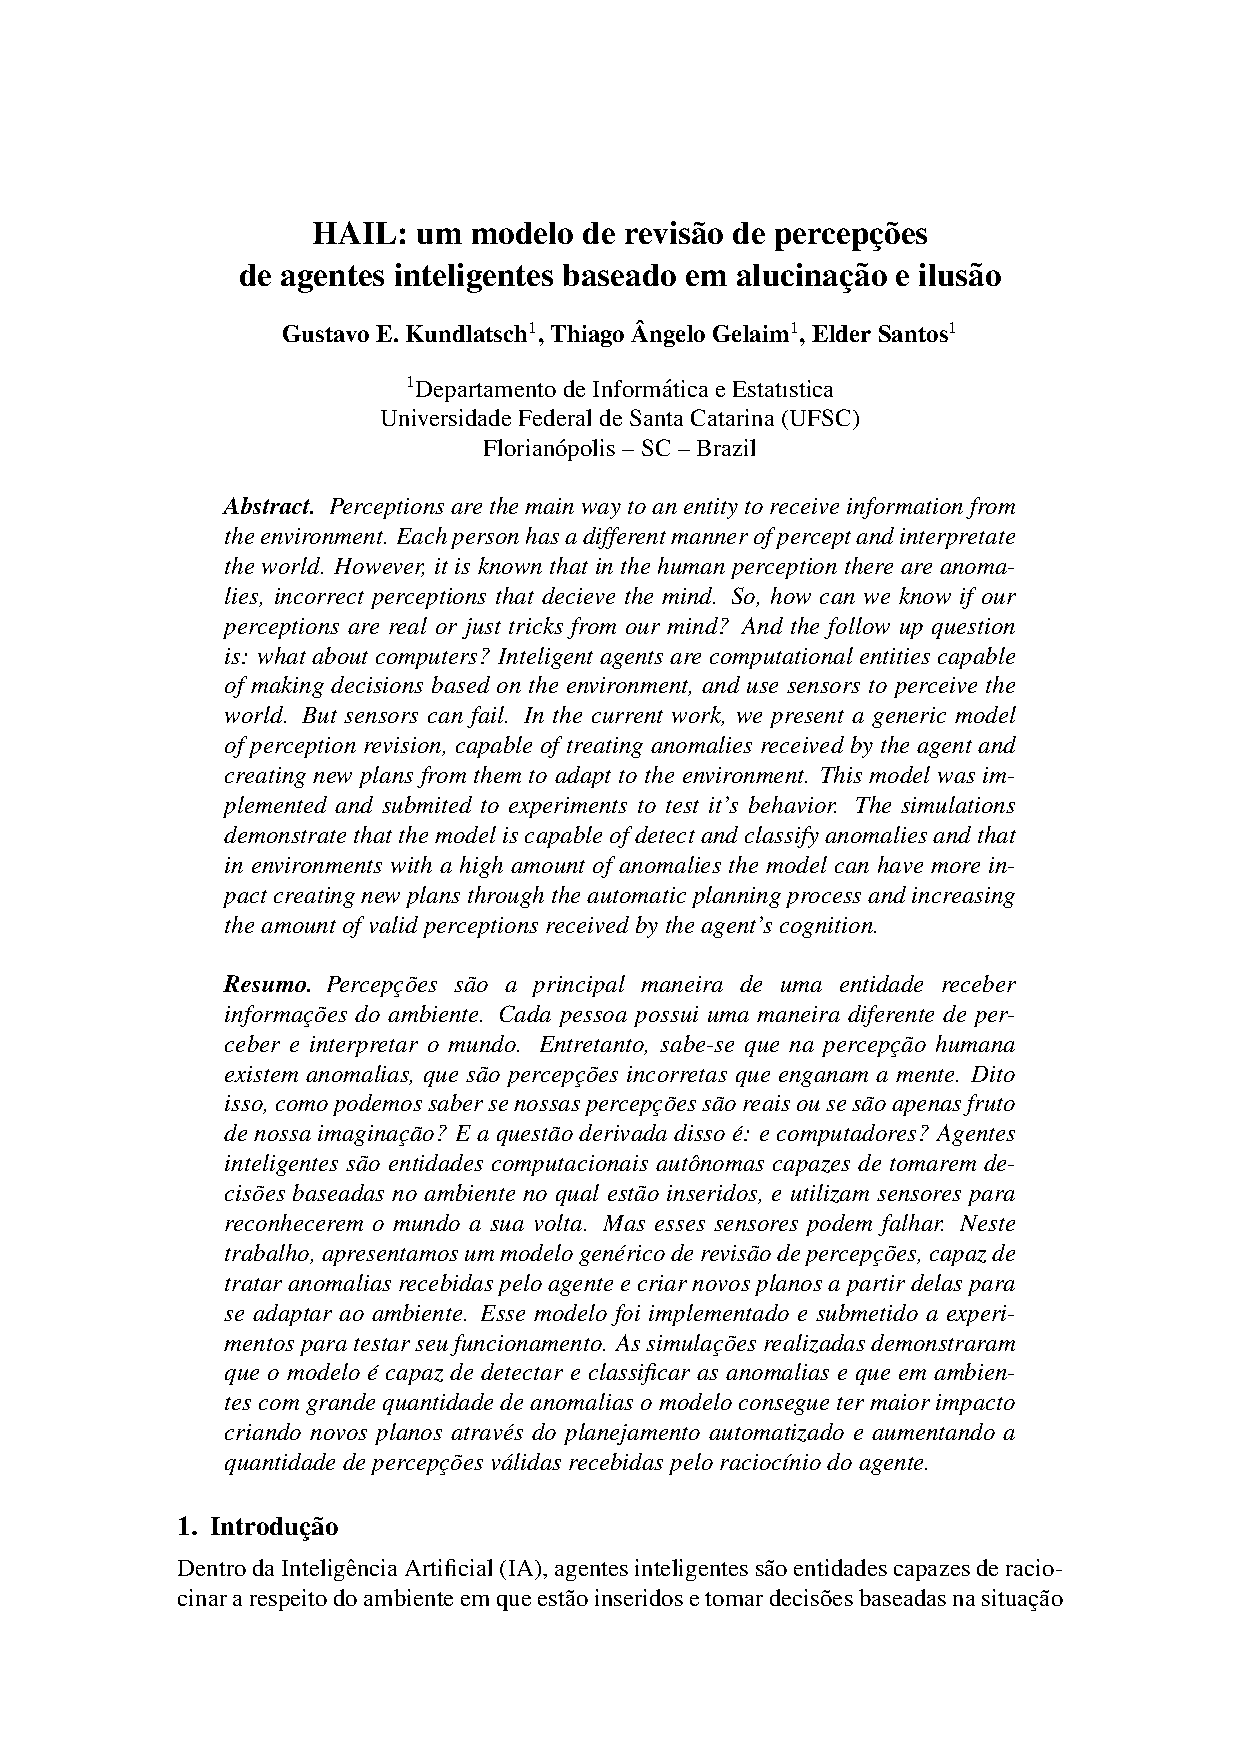
\includepdf[pages=-]{aftertext/Artigo_TCC.pdf}
\end{apendicesenv}
% ---


% ----------------------------------------------------------
% Anexos
% ----------------------------------------------------------

% ---
% Inicia os anexos
% ---
% \begin{anexosenv}
% %	\partanexos*
% 	% ----------------------------------------------------------
\chapter{Descrição 2}
% ----------------------------------------------------------

São documentos não elaborados pelo autor que servem como fundamentação (mapas, leis, estatutos). Deve ser precedido da palavra ANEXO, identificada por letras maiúsculas consecutivas, travessão e pelo respectivo título. Utilizam-se letras maiúsculas dobradas quando esgotadas as letras do alfabeto. 

% \end{anexosenv}

%---------------------------------------------------------------------
% INDICE REMISSIVO
%---------------------------------------------------------------------
%\phantompart
%\printindex
%---------------------------------------------------------------------

\end{document}
